%    minted language=cpp,

%%%%%%
%%%%%%%%%%%%%%%%%%%%%%%%%%%%%% Title Page Info %%%%%%%%%%%%%%%%%%%%%%%%%%%%%%%%%%%%%%%%%%%
%%%%%%%%%%%%%%%%%%%%%%%%%%%%%%%%%%%%%%%%%%%%%%%%%%%%%%%%%%%%%%%%%%%%%%%%%%%%%%%%%%%%%%%%%%

\documentclass[aspectratio=169,compress]{beamer}
\mode<presentation> 

\usetheme{Warsaw}
\usecolortheme[rgb={0.7,0.2,0.0}]{structure}


\usepackage[algosection,lined]{algorithm2e}
\usepackage{minted}
\usepackage{tcolorbox}
\tcbuselibrary{minted}


% define
%\usepackage{beamerouterthememiniframes} % Para los puntitos 
\setbeamertemplate{footline}[frame number]{}

% include packages
\usepackage{subfigure}
\usepackage{multicol}
\usepackage{amsmath}
\usepackage{epsfig}
\usepackage{graphicx}
\usepackage[all,knot]{xy}
\usepackage{algorithmic}
\xyoption{arc}
\usepackage{url}
\usepackage{multimedia}
\usepackage{hyperref}
\usepackage{tikz}

\usepackage{pgfpages}
\setbeameroption{hide notes} % Only slides
%\setbeameroption{show only notes} % Only notes
%\setbeameroption{show notes on second screen=right} % Both




\title{Aplicaciones de visión por computadora desarrolladas en el laboratorio de sistemas inteligentes de la UPV: una retrospectiva} % UPP

\author{Dr. Marco Aurelio Nu\~no Maganda}
\institute{Universidad Politécnica de Victoria\\ Laboratorio de Sistemas Inteligentes \\
mnunom@upv.edu.mx  \vspace{.25cm} }

\date{15 de Noviembre de 2023}
%\textbf{nmaganda@ccc.inaoep.mx}

%%%%%%%%%%%%%%%%%%%%%%%%%%%%%%%%%%%%%%%%%%%%%%%%%%%%%%%%%%%%%%%%%%%%%%%%%%%%%%%%%%%%%%%%%%
%%%%%%%%%%%%%%%%%%%%%%%%%%%%%% Begin Your Document %%%%%%%%%%%%%%%%%%%%%%%%%%%%%%%%%%%%%%%
%%%%%%%%%%%%%%%%%%%%%%%%%%%%%%%%%%%%%%%%%%%%%%%%%%%%%%%%%%%%%%%%%%%%%%%%%%%%%%%%%%%%%%%%%%

 

%\usepackage[backend=biber,maxcitenames=50,maxbibnames=50,sorting=ydmdddnt]{biblatex}
\usepackage[backend=biber,maxcitenames=50,maxbibnames=50,sorting=none]{biblatex}






%\renewrobustcmd{\mkbibfootnote}{\normalsize\footnotemark\footnotetext}
\setbeamerfont{footnote}{size=\tiny}






\newcommand{\ArchivoPrincipal}{Todos}
\newcommand{\ArchivoSecundario}{Bibliografia}


%Append keywords to identify different bibliography entries.
\DeclareSourcemap{
  \maps[datatype=bibtex, overwrite]{
    \map{
      \perdatasource{\ArchivoPrincipal.bib}
      \step[fieldset=KEYWORDS, fieldvalue=primary, append]
    }
    \map{
      \perdatasource{\ArchivoSecundario.bib}
      \step[fieldset=KEYWORDS, fieldvalue=secundary, append]
    }    
  }
}


\addbibresource{\ArchivoPrincipal.bib}
\addbibresource{\ArchivoSecundario.bib}

\usepackage{listings}
 
 \AtBeginSection[]
{
    \begin{frame}
        \frametitle{Outline}
        \tableofcontents[currentsection]
    \end{frame}
}

\makeatletter
\def\@makefnmark{}
\makeatletter
\setbeamertemplate{footnote}{%
  \parindent 1em\noindent
  \raggedright
  *  
  \insertfootnotetext\par
}

% ACtualizacion 2024: Se necesita esta Entrada
\newcommand{\EntradaBibtex}{InvalidEntry}


\begin{document}

\frame{
	%\titlepage 
	\begin{titlepage}
	\end{titlepage}
	
}



\frame{
\frametitle{Contenido}
\tableofcontents
}

\section{2012}
% SCRIPT
% The next project in this presentation is named "A Novel Strategy for Image Segmentation of Latent Fingerprints~}." 
% The results of this project were published on a confence paper in 2012. 
% Slide 1




% Slide 2


% Slide 3

% Conclusion

%\renewcommand{\Titulo}{A Novel Strategy for Image Segmentation of Latent Fingerprints~}


\begin{frame}{\citetitle{MarcoNuno_CongArbIng_2012_02_00} \footnotemark (1)}

\note[item]{\scriptsize  A Fingerprint is an impression or mark made on a surface by a person's fingertip, especially as used for identifying individuals from the unique pattern of whorls and lines.}
\note[item]{\scriptsize  The main stages of AFIS involves:  1. Capture of the fingerprint image. 2. Image processing 3. Feature extraction  4. Matching 5. Storing}
%\note[item]{\scriptsize  The adequate processing of the fingerprint image is a relevant task for the recognition process. If the image is not processed correctly, false characteristics could be obtained in the feature extraction phase or important information could be discarded, increasing the probability that the identification of the individual and the system fails.}
\note[item]{\scriptsize  In this project a new strategy for segmentation of latent fingerprints is proposed, based on the use of gradients and the detection of regions in the image. Our algorithm is able to detect the area of interest in the fingerprint eliminating spots, shadows, noise, etc., and adapting itself to the different conditions in the image.}

	\begin{itemize}
\item Automatic Fingerprint Identification Systems (AFIS) are very important due to their security applications.
\item The main stages of AFIS involves several image processing operators. 
\item The adequate processing of the fingerprint image is important 

	\end{itemize}
	    \begin{center}
    \begin{tabular}{c}
        \includegraphics[width=0.75\linewidth]{Figs/Fingerprint1}\\
    \end{tabular}
    	    \end{center}

\footnotetext[1]{\fullcite{MarcoNuno_CongArbIng_2012_02_00}}
\setcounter{footnote}{0}
\end{frame}

\begin{frame}{\citetitle{MarcoNuno_CongArbIng_2012_02_00} (2)}
Estrategia propuesta:
\begin{columns}
		\begin{column}{0.48\textwidth}

		    \begin{enumerate} \small
		        \item Compute gradient and gradient magnitude.
                \item Normalize the pixel values to the range [0 255].
                \item Binarize the normalized image.
                \item Apply a mean filter to the binarized image            
            \end{enumerate}  
        \end{column}          
		\begin{column}{0.48\textwidth}
		    \begin{enumerate} \small
				\setcounter{enumi}{4}
    \item Binarize the image obtained
                \item Find the label matrix.
                \item Find the label with the high number of instances.
                \item Detect the largest region of interest.			
            \end{enumerate}  

        \end{column}
\end{columns}


\note[item]{\scriptsize  The gradient is a tool widely used for detecting edges in
an image. 
}

%\note[item]{\scriptsize This normalization is performed executing the following steps: ii) Find the minimum intensity value. ii) Subtract the minimum intensity value to each pixel in the image. iii) Find the maximum intensity value in the image and divide 255 by it. iv) Multiply each intensity value by the result obtained in the previous step.}

\note[item]{\scriptsize Binarize the normalized image using as threshold the
mean value of the gradient magnitude image.}

%\note[item]{\scriptsize A new median value is computed from the binarized image, which will be used as threshold for future binarization}

\note[item]{\scriptsize  The labeling algorithm allows to identify zones in the input image formed by interconnected pixels in a binary image that belongs to the foreground (object of interest).}

%\note[item]{\scriptsize Excluding labels that belongs to the background.}

%\note[item]{\scriptsize Send to the background the rest of the detected regions.}

		
\begin{center}
     \begin{tabular}{c}
         \includegraphics[width=0.95\linewidth]{Figs/Fingerprint2}\\
          \end{tabular}
\end{center}


\end{frame}

\begin{frame}{\citetitle{MarcoNuno_CongArbIng_2012_02_00} (2)}

\note[item]{\scriptsize  In this slide we show the different stages of the segmentation strategy proposed in this work. }

\note[item]{\scriptsize The resolution of images used in this work is 328 × 364 pixels .}

%Resultados
\begin{columns}
		\begin{column}{0.48\textwidth}
		We compared the proposed method against the most representative segmentation algorithms
		\begin{itemize}
		\item Our method achieves the better results, producing as result of
segmentation a single region and discarding no relevant information in the latent fingerprint.
    \item Images that have high contrast between the peaks and valleys that remark the borders in the image performs better.
				\end{itemize}
        \end{column}
				\begin{column}{0.48\textwidth}
				
\begin{center}
     \begin{tabular}{c}
              \includegraphics[width=0.85\textwidth]{Figs/Fingerprint3}
          \end{tabular}
\end{center}
				\end{column}
								\end{columns}

\end{frame}











\section{2014}




\begin{frame}{\citetitle{MarcoNuno_CongArbIng_2014_12_00X}  \footnotemark (1)}
\begin{columns}
\begin{column}{0.4\textwidth}
		Componentes:
		\begin{itemize}
		\item Una cama para libros abiertos
		\item Un mecanismo para cambiar de página a través de uns servomotores
		\item Un sistema de iluminación 		
		\end{itemize}
\end{column}
\begin{column}{0.6\textwidth}  
    \begin{center}
     %%%%% this is a minipage, so \textwidth is already adjusted to the size of the column
     \includegraphics[width=0.8\textwidth]{Figs/BookScanner1}
     \end{center}
\end{column}
\end{columns}

\footnotetext[1]{\fullcite{MarcoNuno_CongArbIng_2014_12_00X}}
\setcounter{footnote}{0}
\end{frame}


\begin{frame}{\citetitle{MarcoNuno_CongArbIng_2014_12_00X} (2)}
%\begin{block}{Prototipo para Digitalizar Libros (2)} 
\begin{columns}
\begin{column}{0.6\textwidth}
		\begin{itemize}
		\item Una cámara de alta definición para capturar fotografías de ambas páginas
		\item Una computadora Embebida con la cámara conectada para procesar la imágen e integrar el libro digitalizado en formato PDF.
		\item Nucleo: Un sistema de visión para detectar automáticamente los límites de las páginas y cortas para generar el documento
		\end{itemize}
\end{column}
\begin{column}{0.4\textwidth}  
    \begin{center}
     %%%%% this is a minipage, so \textwidth is already adjusted to the size of the column
     \includegraphics[width=0.8\textwidth]{Figs/BookScanner2}
     \end{center}
\end{column}
\end{columns}
%\end{block} 
\end{frame}


\begin{frame}{\citetitle{MarcoNuno_CongArbIng_2014_12_00X} (3)}
%\begin{block}{} 
\begin{columns}
\begin{column}{0.5\textwidth}
%   some text here some text here some text here some text here some text here
     \begin{center}
     %%%%% this is a minipage, so \textwidth is already adjusted to the size of the column
     \includegraphics[width=0.88\textwidth]{Figs/BookScanner3}
     \end{center}

\end{column}
\begin{column}{0.5\textwidth}  
    \begin{center}
     %%%%% this is a minipage, so \textwidth is already adjusted to the size of the column
     \includegraphics[width=0.88\textwidth]{Figs/BookScanner4}
     \end{center}
\end{column}
\end{columns}
%\end{block} 
\end{frame}




\begin{frame}{\citetitle{MarcoNuno_CongArbEsp_2014_09_02}$^*$  (1)}
\begin{columns}
\begin{column}{0.6\textwidth}
	\begin{itemize}
		\item El estudiante había trabajado en CAPUFE
        \item Tener un mecanismo que evitara que los vehiculos pagaran menos peaje debido a errores de registro
		\item Contar de manera automática el número de ejes de los vehículos
	\end{itemize}
\end{column}
\begin{column}{0.4\textwidth}  
\begin{center}
     \begin{tabular}{c}
\includegraphics[width=0.68\textwidth]{2014_Llantas/figs/LuisRodolfo1}\\
\includegraphics[width=0.68\textwidth]{2014_Llantas/figs/LuisRodolfo2}\\         
      \end{tabular}
\end{center}
\end{column} 
\end{columns} 
\footfullcite*{MarcoNuno_CongArbEsp_2014_09_02}
\end{frame}


\begin{frame}{\citetitle{MarcoNuno_CongArbEsp_2014_09_02} (2)}
	\begin{itemize}
        \item Detectar el vehiculo
        \item Acotar las zonas de interes
        \item Aplicar filtrado a los frames individuales
        \item Detectar contornos para reducir la región de búsqueda de las regiones circulares
        \item Aplicar detección de circulos y generar como resultado el número de ejes
	\end{itemize}
\begin{center}
 \begin{tabular}{cccc}
    \includegraphics[width=5cm]{2014_Llantas/figs/LuisRodolfo5}
    \includegraphics[width=4cm]{2014_Llantas/figs/LuisRodolfo3}
    \includegraphics[width=4cm]{2014_Llantas/figs/LuisRodolfo4}
  \end{tabular}
\end{center}

\end{frame}











%\section{Proyectos de Investigación}
%\subsection{Visión por Computadora}
\begin{frame}{\citetitle{MarcoNuno_CongArbIng_2014_07_00}}
\begin{block}{} 
\begin{columns}
\begin{column}{0.4\textwidth}
		\begin{itemize}
		\item Detección y conteo de autómoviles 
		\item Videos capturados desde pueden peatonales
		\item  Detectar regiones de movimiento 
		\end{itemize}
\end{column}
\begin{column}{0.6\textwidth}  
    \begin{center}
     %%%%% this is a minipage, so \textwidth is already adjusted to the size of the column
     \includegraphics[width=0.70\textwidth]{Figs/TrafficFlow}
     \end{center}
\end{column}
\end{columns}
\end{block} 
%\footnotetext{Raul Humberto Peña-González and Marco Aurelio Nuño-Maganda. \textbf{Computer vision based real-time vehicle tracking and classification system}. In 2014 IEEE 57th International Midwest Symposium on Circuits and Systems (MWSCAS 2014), pages 679–682, Agosto 2014. http://doi.org/10.1109/MWSCAS.2014.6908506ISBN: 978-1-4799-4132-2}
\footnotetext[1]{\fullcite{MarcoNuno_CongArbIng_2014_07_00}}
\setcounter{footnote}{0}


\end{frame}

\begin{frame}{Proyectos de Investigación}
\begin{block}{Seguimiento y Clasificación de Vehículos (2)} 
\begin{columns}
\begin{column}{0.4\textwidth}
		\begin{itemize}
		\item Se capturaron videos de diferentes ubicaciones
		\item Se estimó la densidad de flujo de trafico y por tipo de vehiculo
		\item Idea original: detectar conductores usando telefono celular al manejar
		\end{itemize}
\end{column}
\begin{column}{0.6\textwidth}  
    \begin{center}
     %%%%% this is a minipage, so \textwidth is already adjusted to the size of the column
     \includegraphics[width=0.8\textwidth]{Figs/TrafficFlow2}
     \end{center}
\end{column}
\end{columns}
\end{block} 
\setcounter{footnote}{0}
\end{frame}








\section{2020}




%\begin{frame}{Proyectos de Investigación}
\begin{frame}{\citetitle{MarcoNuno_Revista_2020_04_00} \footnotemark (1)}
\begin{columns}
\begin{column}{0.70\textwidth}
Propuesta:
		\begin{itemize}
		\item Un \textit{Cariograma} es una representación ordenada de los cromosomas.  
		\item Un \textit{Citogenetista} es una experto que diagnotisca enfermedades genéticas a partir de Cariograma.		
		\item Un sistema que auxilie al Citogenetista a crear el Cariograma de forma automática.
		\item Se requieren técnicas de visión por computadora y aprendizaje automáticos.
		\end{itemize}
\end{column}
\begin{column}{0.30\textwidth}  
    \begin{center}
     %%%%% this is a minipage, so \textwidth is already adjusted to the size of the column
     \includegraphics[width=0.98\textwidth]{Figs/Karyogram1}
     \includegraphics[width=0.98\textwidth]{Figs/Karyogram2}
     \end{center}
\end{column}
\end{columns}
\footnotetext[1]{\fullcite{MarcoNuno_Revista_2020_04_00}}
\setcounter{footnote}{0}
\end{frame}


\begin{frame}{\citetitle{MarcoNuno_Revista_2020_04_00} \footnotemark (2)}
\begin{columns}
\begin{column}{0.6\textwidth}
Pasos a aplicar:
		\begin{enumerate}
		\item Segmentación de los cromosomas individuales 
		\item Extracción de características
		\item Clasificación por tamaño
		\item Clasificación por tipo dentro de cada tamaño
		\item Integración
		\item Construcción del Cariograma
		\end{enumerate}
    \begin{center}
     %%%%% this is a minipage, so \textwidth is already adjusted to the size of the column
     \includegraphics[width=0.5\textwidth]{Figs/Karyogram4}
     \end{center}


\end{column}
\begin{column}{0.4\textwidth}  
    \begin{center}
     %%%%% this is a minipage, so \textwidth is already adjusted to the size of the column
     \includegraphics[width=0.7\textwidth]{Figs/Karyogram5}
     \end{center}
\end{column}
\end{columns}
\end{frame}






   

\begin{frame}{\citetitle{MarcoNuno_Revista_2020_06_00} \footnotemark (1)}
\begin{block}{Sistema de Monitoreo de Aprendizaje Remoto } 

Con la reciente pandemia, se detectan problemas con el seguimiento del aprendizaje:

	\begin{itemize}
		\item No es posible determinar si el estudiante es quien realiza las tareas
		\item No hay certeza de que tanto tiempo el estudiante dedica a ciertas tareas
	\end{itemize}

Se propone una herramienta cuyos componentes son:
\begin{itemize}
\item Aplicación de Escritorio - El docente asigna tareas·
\item Aplicación en la NUBE - Almacena tareas y evidencias (fotos).
\item Aplicación de Móvil - Monitorea al estudiante emplenado la cámara frontal del teléfono inteligente, además le permite recopilar evidencias.
\end{itemize}
\end{block} 
\footnotetext[1]{\fullcite{MarcoNuno_Revista_2020_06_00}}
\setcounter{footnote}{0}
\end{frame}

\begin{frame}{\citetitle{MarcoNuno_Revista_2020_06_00} (2)}


\begin{columns}
\begin{column}{0.65\textwidth}
\begin{block}{La aplicación de escritorio:} 
		\begin{itemize}
		\item Permite crear grupos, tareas, dar de alta alumnos
		\item Descargar evidencias
		\item Generar una gráfica de tiempo de atención
		\end{itemize}
\end{block} 
\begin{block}{La aplicación móvil:} 
		\begin{itemize}
		\item Recibe las tareas y las muestra al alumno
		\item Monitorea al estudiante a lo largo del desarrollo de sus tareas
		\end{itemize}
\end{block} 
\end{column}
\begin{column}{0.35\textwidth}  
    \begin{center}
     %%%%% this is a minipage, so \textwidth is already adjusted to the size of the column
     \includegraphics[width=0.95\textwidth]{Figs/LearningMonitoring1}
     \includegraphics[width=0.95\textwidth]{Figs/LearningMonitoring2}
     \end{center}
\end{column}
\end{columns}


\end{frame}

\begin{frame}{\citetitle{MarcoNuno_Revista_2020_06_00} (3)}


\begin{columns}
\begin{column}{0.5\textwidth}
\begin{block}{Pasos ejecutados por la App: } 
		\begin{itemize}
		\item Detecta la cara del estudiante y estima hacia donde esta mirando (la pantalla, el área de trabajo o el exterior)
		\item Detecta cuando el estudiante cierra la aplicación y lleva la cuenta del tiempo que la aplicación de monitoreo permanece inactiva. 
		\end{itemize}
\end{block} 
	\begin{center}
		 \includegraphics[width=0.50\textwidth]{Figs/LearningMonitoring3}
	\end{center}
\end{column}
\begin{column}{0.5\textwidth}  
    \begin{center}
     %%%%% this is a minipage, so \textwidth is already adjusted to the size of the column
     \includegraphics[width=0.99\textwidth]{Figs/LearningMonitoring4}
     \end{center}
\end{column}
\end{columns}

%\end{block} 
\end{frame}


          




\begin{frame}{\citetitle{MarcoNuno_CongArbEsp_2020_09_01} \footnotemark (1)}
\begin{block}{Detección de conductores autorizados \footnotemark } 
\begin{columns}
\begin{column}{1.0\textwidth}
Se propone un sistema montado en un teléfono inteligente que pueda:
	\begin{itemize}
\item Confirmar de manera continua la identidad de los ocupantes empleando la cámara frontal o posterior
\item Monitorear la ubicación del vehículo mediante el sensor GPS
\item Monitorear cuando el vehículo está en movimiento mediante los acelerómetros
\item Trabajar de manera independiente, conectado continuamente a la corriente y con conexión de datos propia para comunicación externa
	\end{itemize}
\end{column}
\end{columns}
\end{block} 
\footnotetext[1]{\fullcite{MarcoNuno_CongArbEsp_2020_09_01}}
\setcounter{footnote}{0}
\end{frame}


\begin{frame}{\citetitle{MarcoNuno_CongArbEsp_2020_09_01} (2)}
%\begin{block}{Detección de conductores autorizados (2)} 
\begin{columns}
\begin{column}{0.55\textwidth}
Fases de la ejecución:
	\begin{enumerate}
\item Enrolamiento: Los usuarios usan el automovil y sus rostros quedan guardados.
\item Prueba: Se reporta el ingreso de cualquier extraño.
	\end{enumerate}
Limitaciones:
	\begin{itemize}
\item Solo piloto, copiloto y tal vez pasajero viajando en el centro de la parte posterior.
\item Iluminación diurna.
\item Camuflaje en fase temprana.
	\end{itemize}

\end{column}
\begin{column}{0.45\textwidth}
\begin{center}
     %%%%% this is a minipage, so \textwidth is already adjusted to the size of the column
     \includegraphics[width=0.99\textwidth]{Figs/ConductorAutorizado1}
     \end{center}
\end{column}

\end{columns}
%\end{block} 
\end{frame}





\section{2021}
\begin{frame}{Detección de movimientos en un tablero de ajedrez \footnotemark}
%\begin{block}{Detección de movimientos en un tablero de ajedrez \footnotemark} 
\begin{columns}
\begin{column}{0.38\textwidth}
Aplicación de escritorio:
	\begin{itemize}
\item Entorno semicontrolado con una cámara y una Laptop con OpenCV
\item Detecta las esquinas del tablero de ajedrez
\item Transformada de Hough
\item Detectar si hay casilla o no dentro de la región de interés
	\end{itemize}
\end{column}
\begin{column}{0.28\textwidth}
\begin{center}
     %%%%% this is a minipage, so \textwidth is already adjusted to the size of the column
     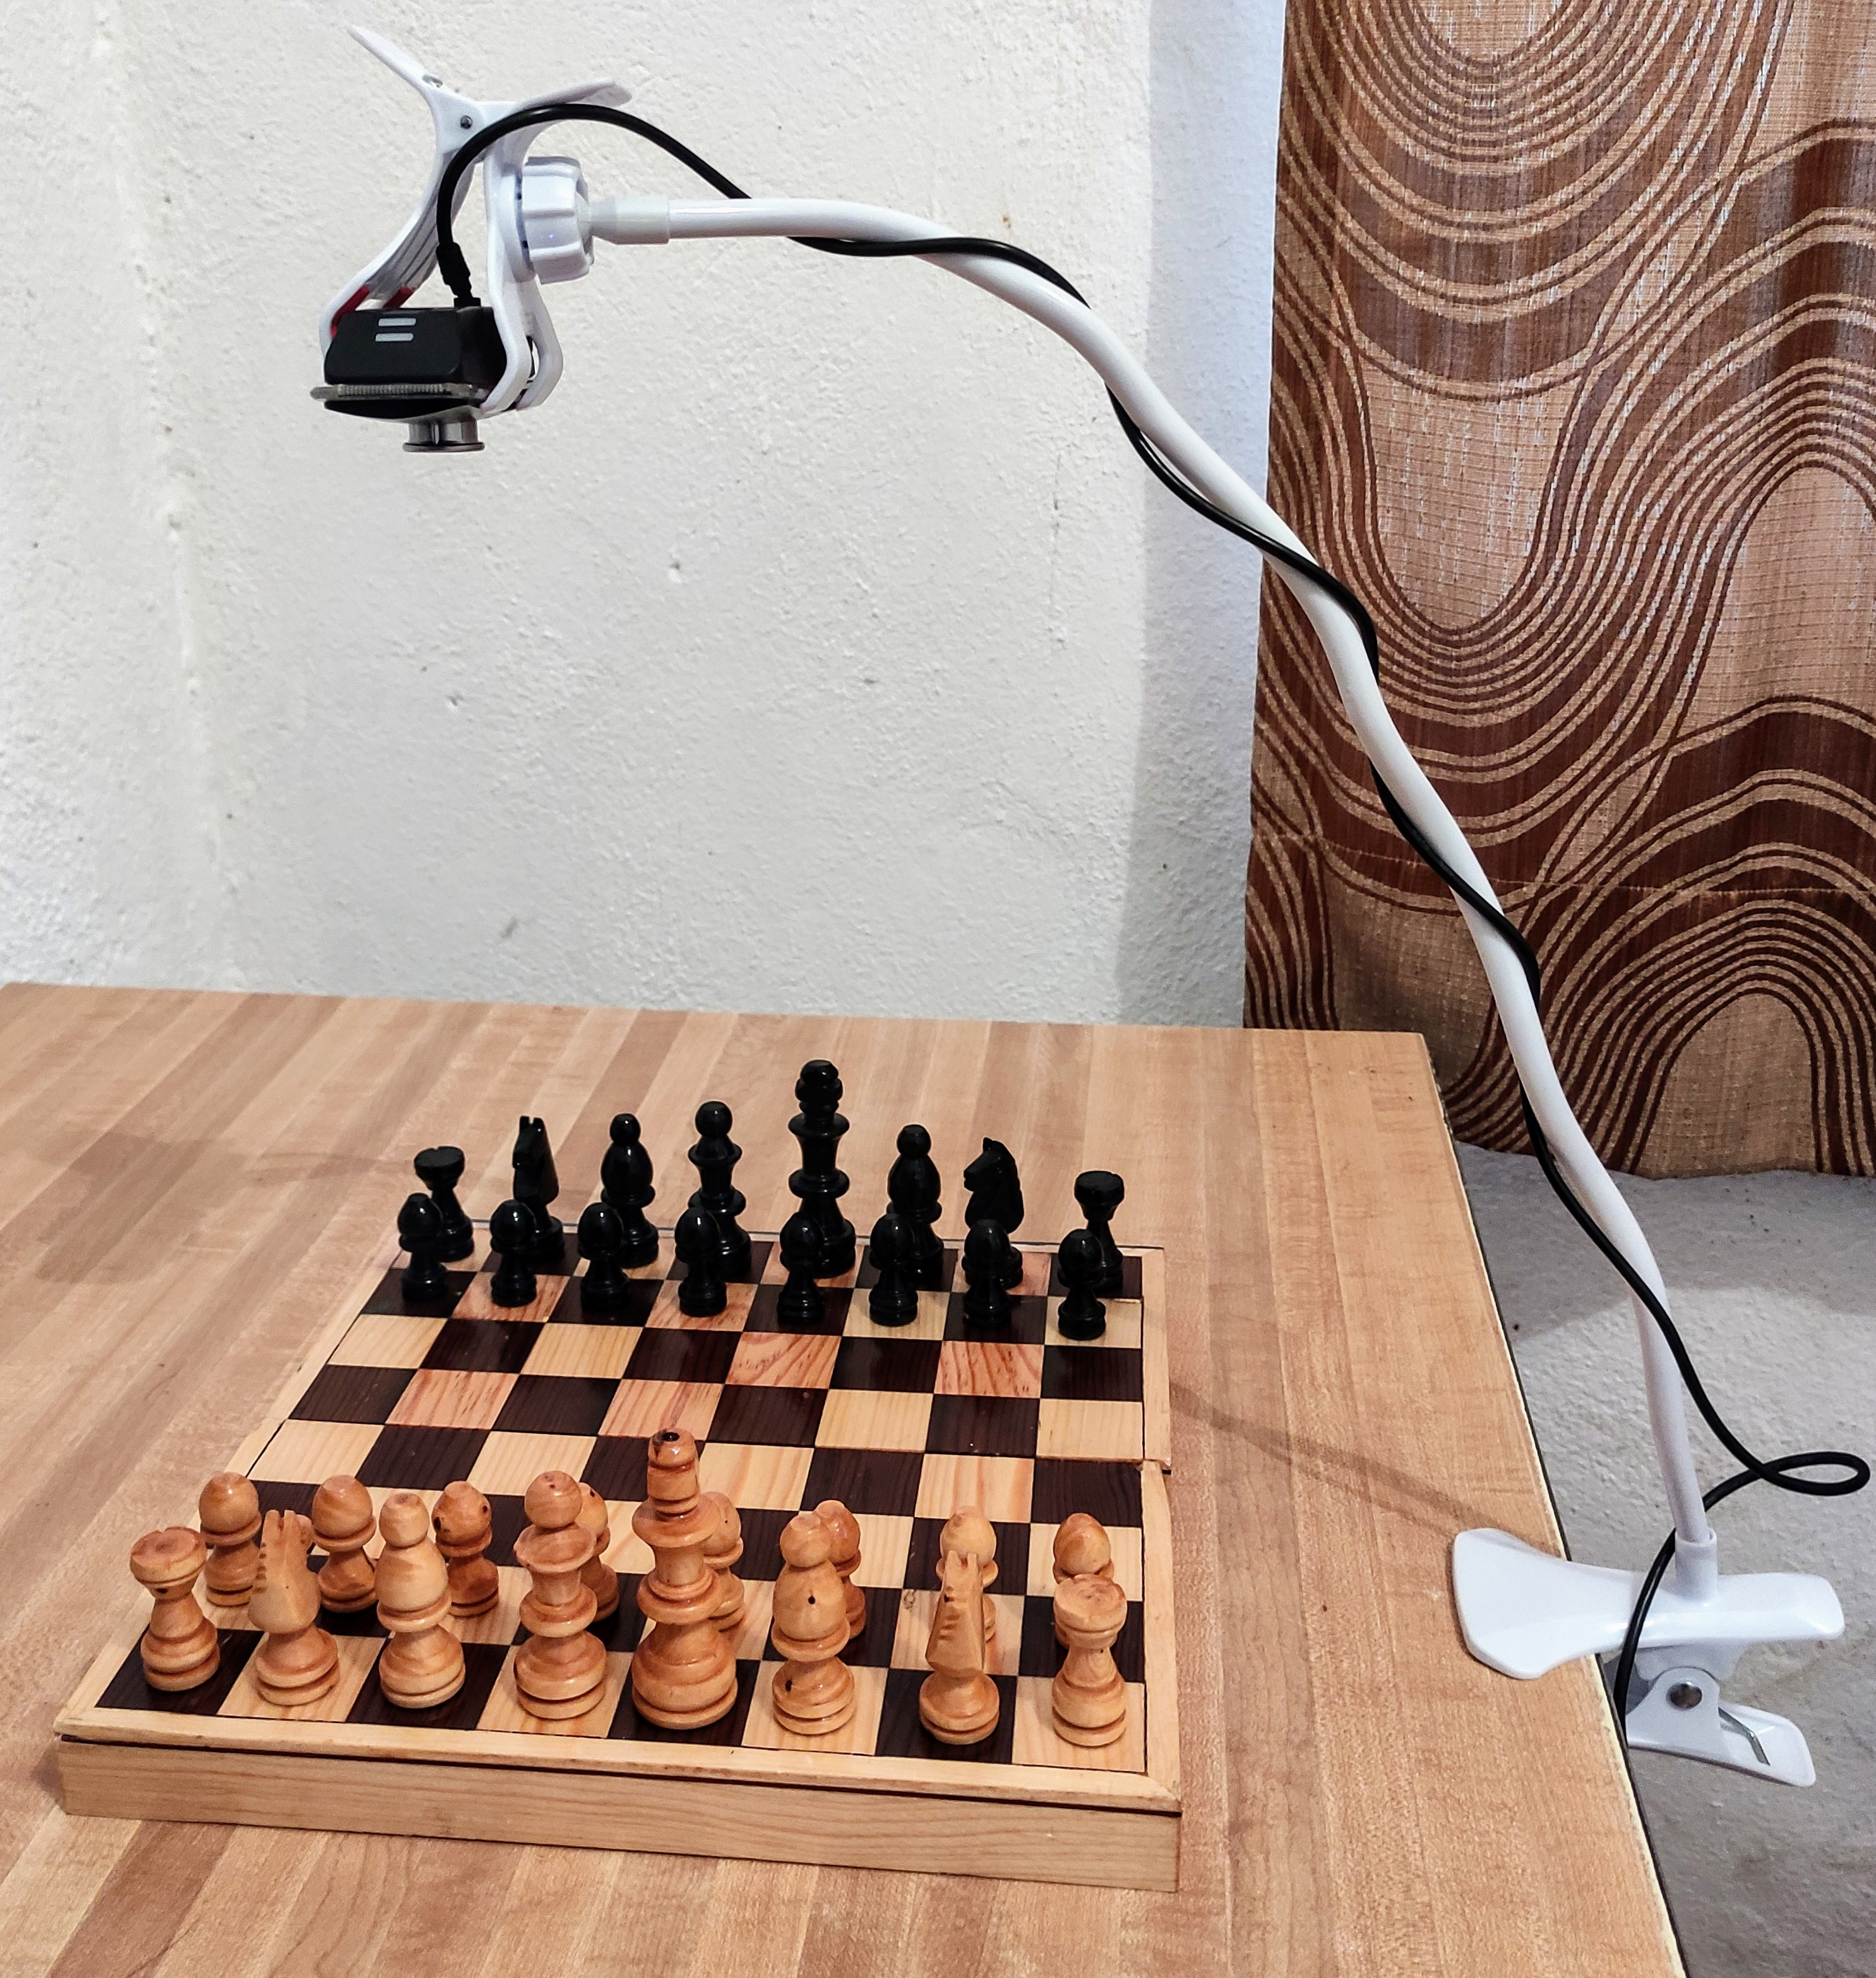
\includegraphics[width=0.75\textwidth]{Figs/AjedrezFroylan1}\\
%     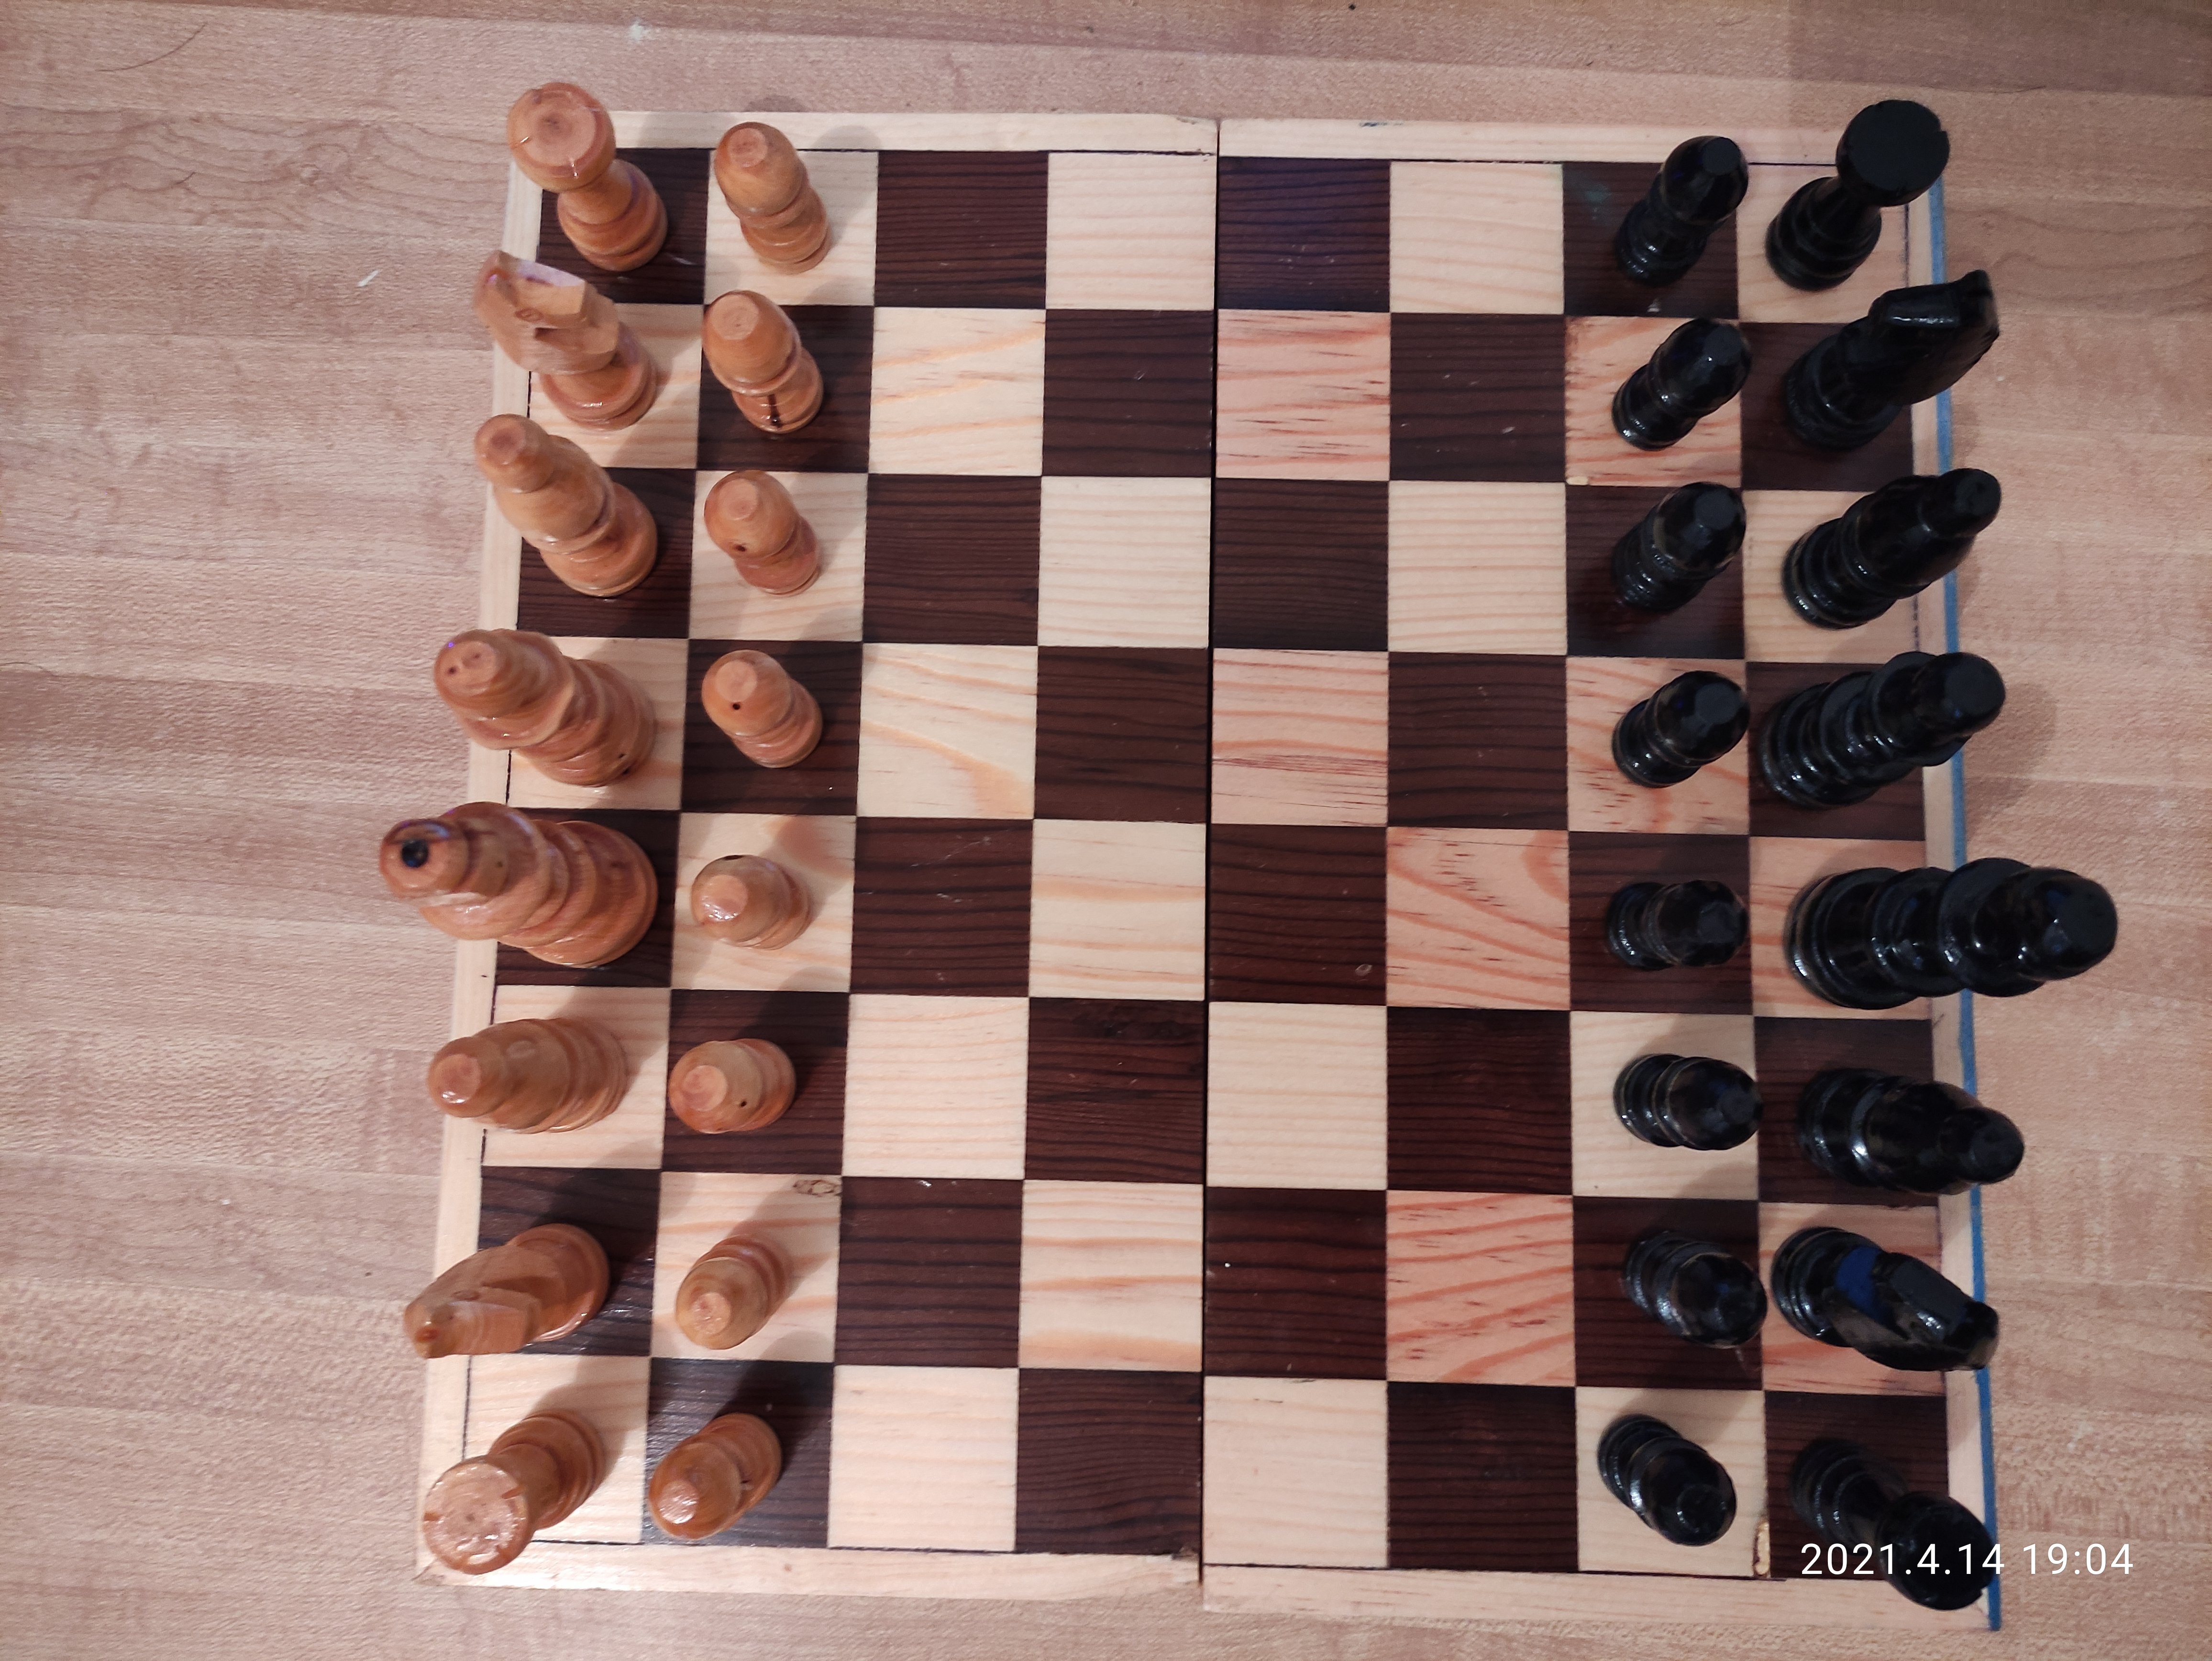
\includegraphics[width=0.35\textwidth]{Figs/AjedrezFroylan2}
     \end{center}
\end{column}
\begin{column}{0.28\textwidth}
\begin{center}
     %%%%% this is a minipage, so \textwidth is already adjusted to the size of the column
 %    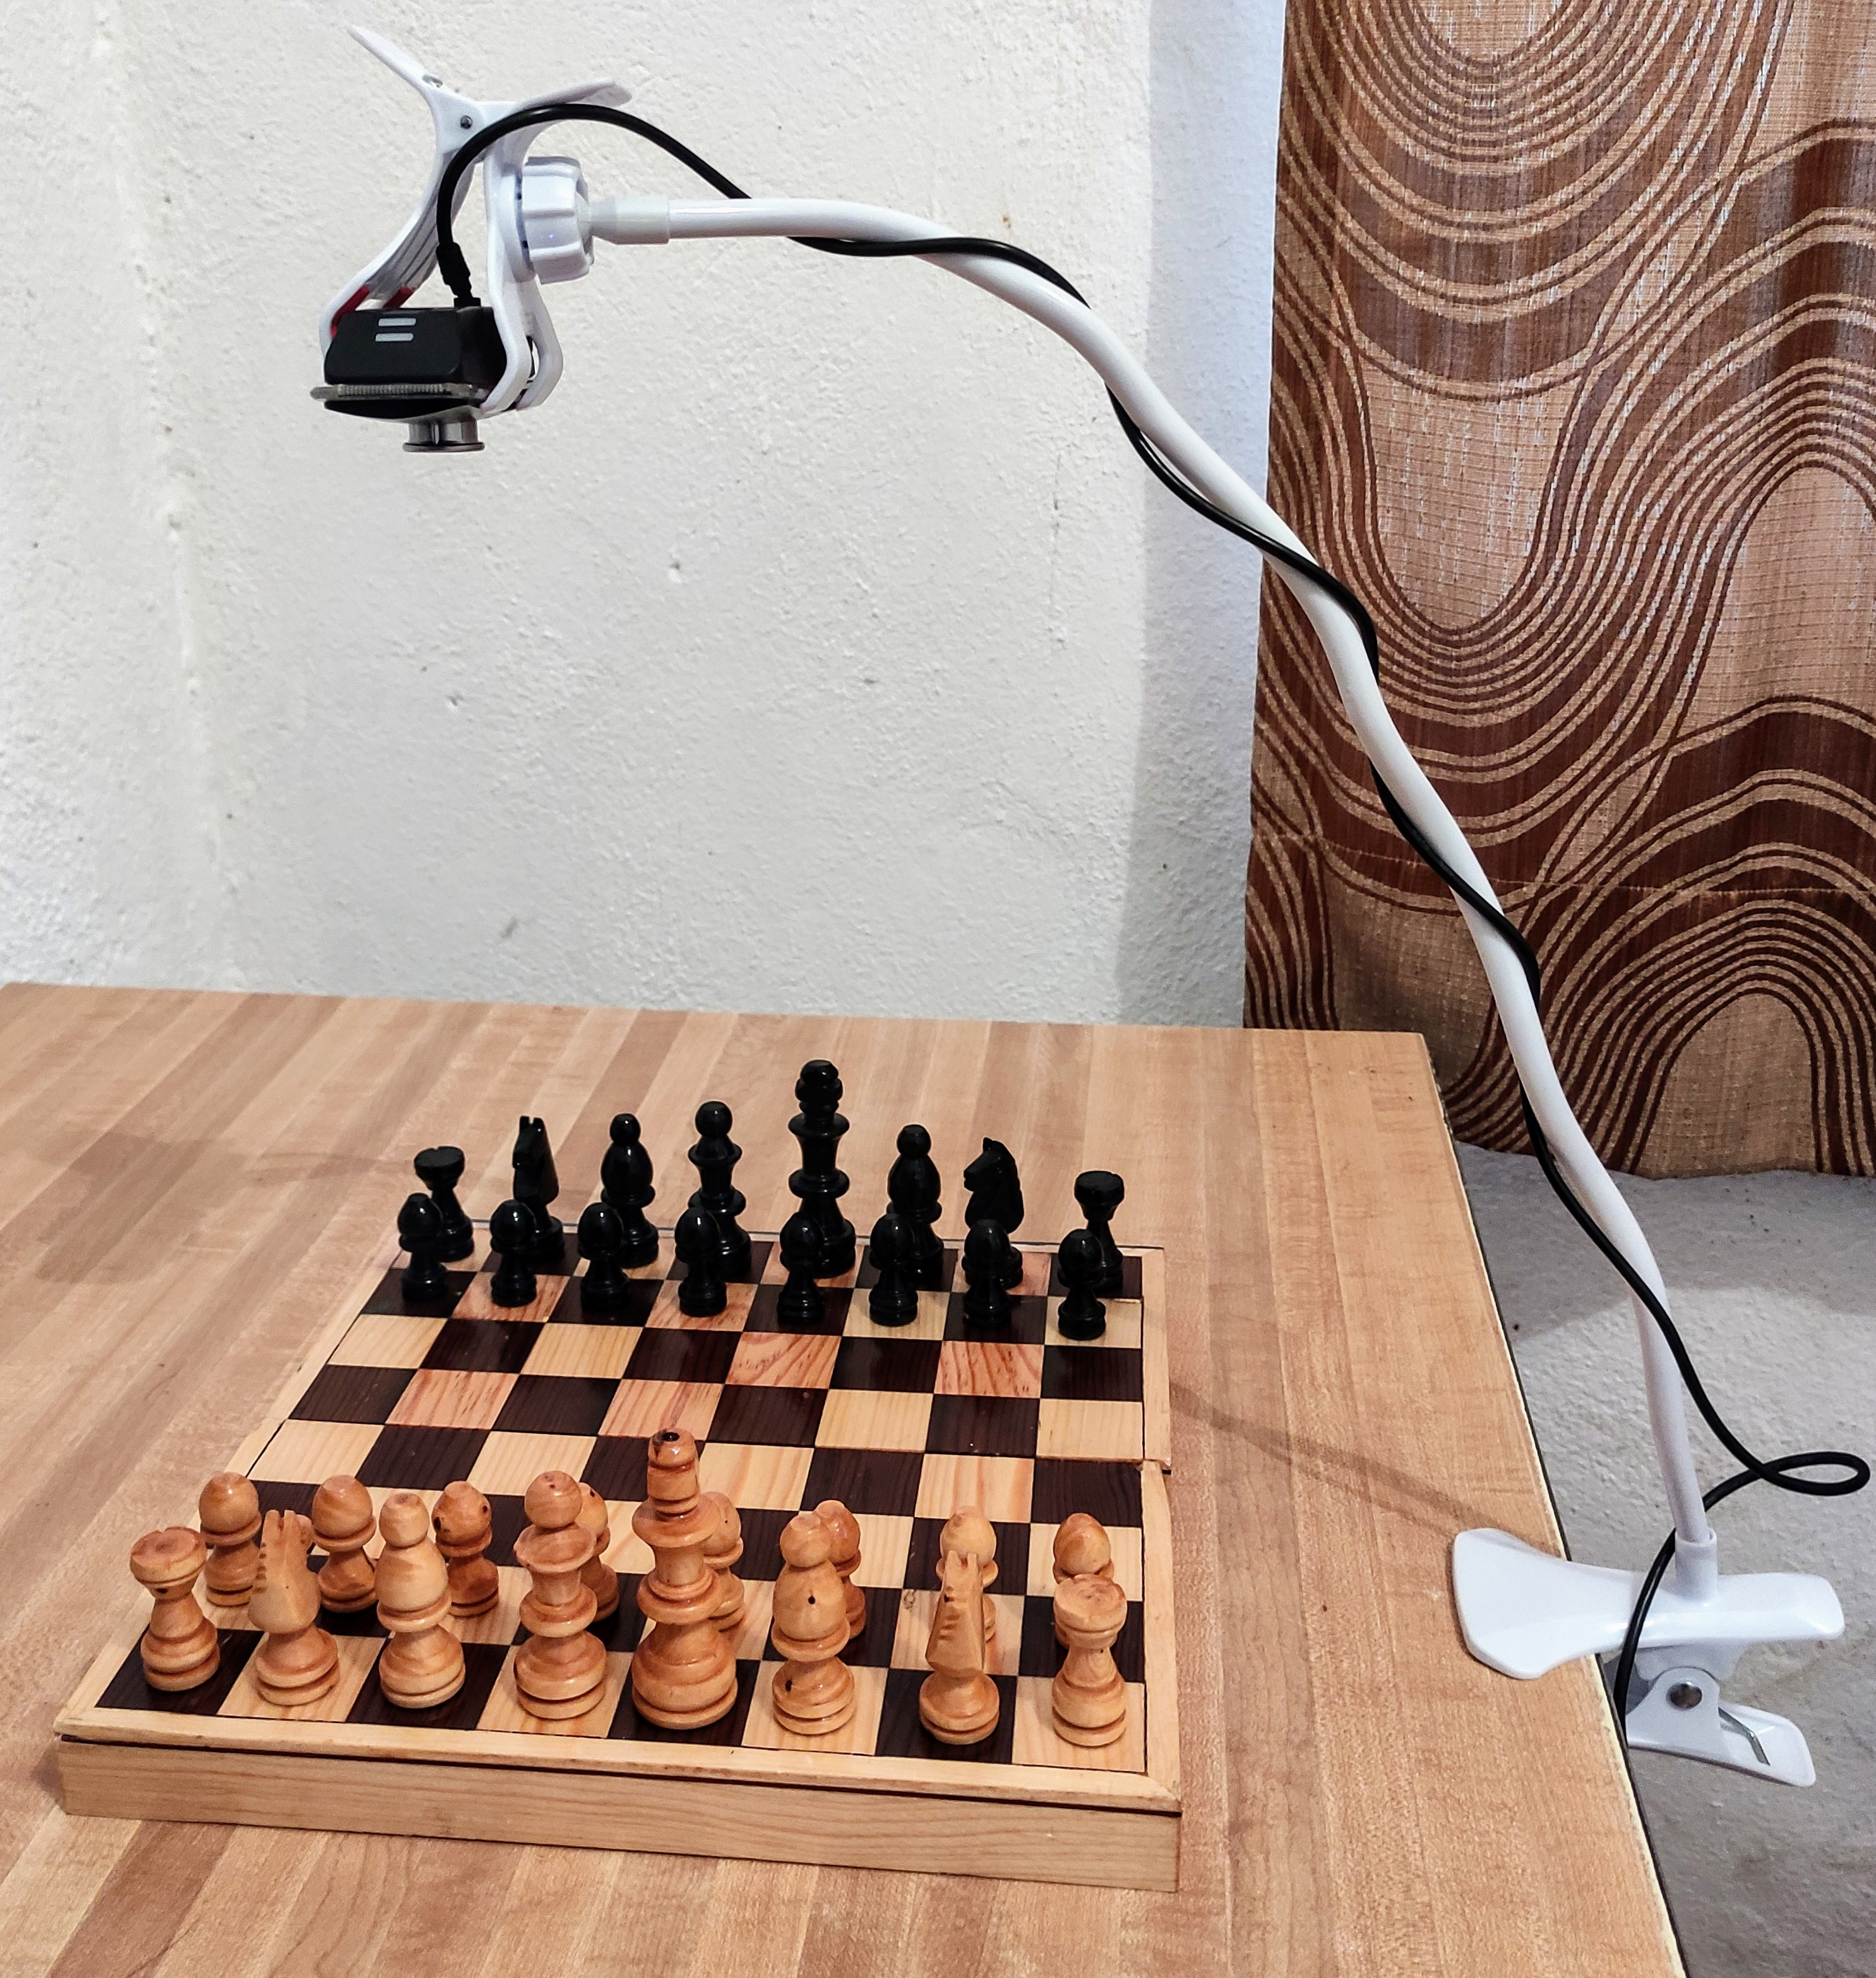
\includegraphics[width=0.35\textwidth]{Figs/AjedrezFroylan1}\\
     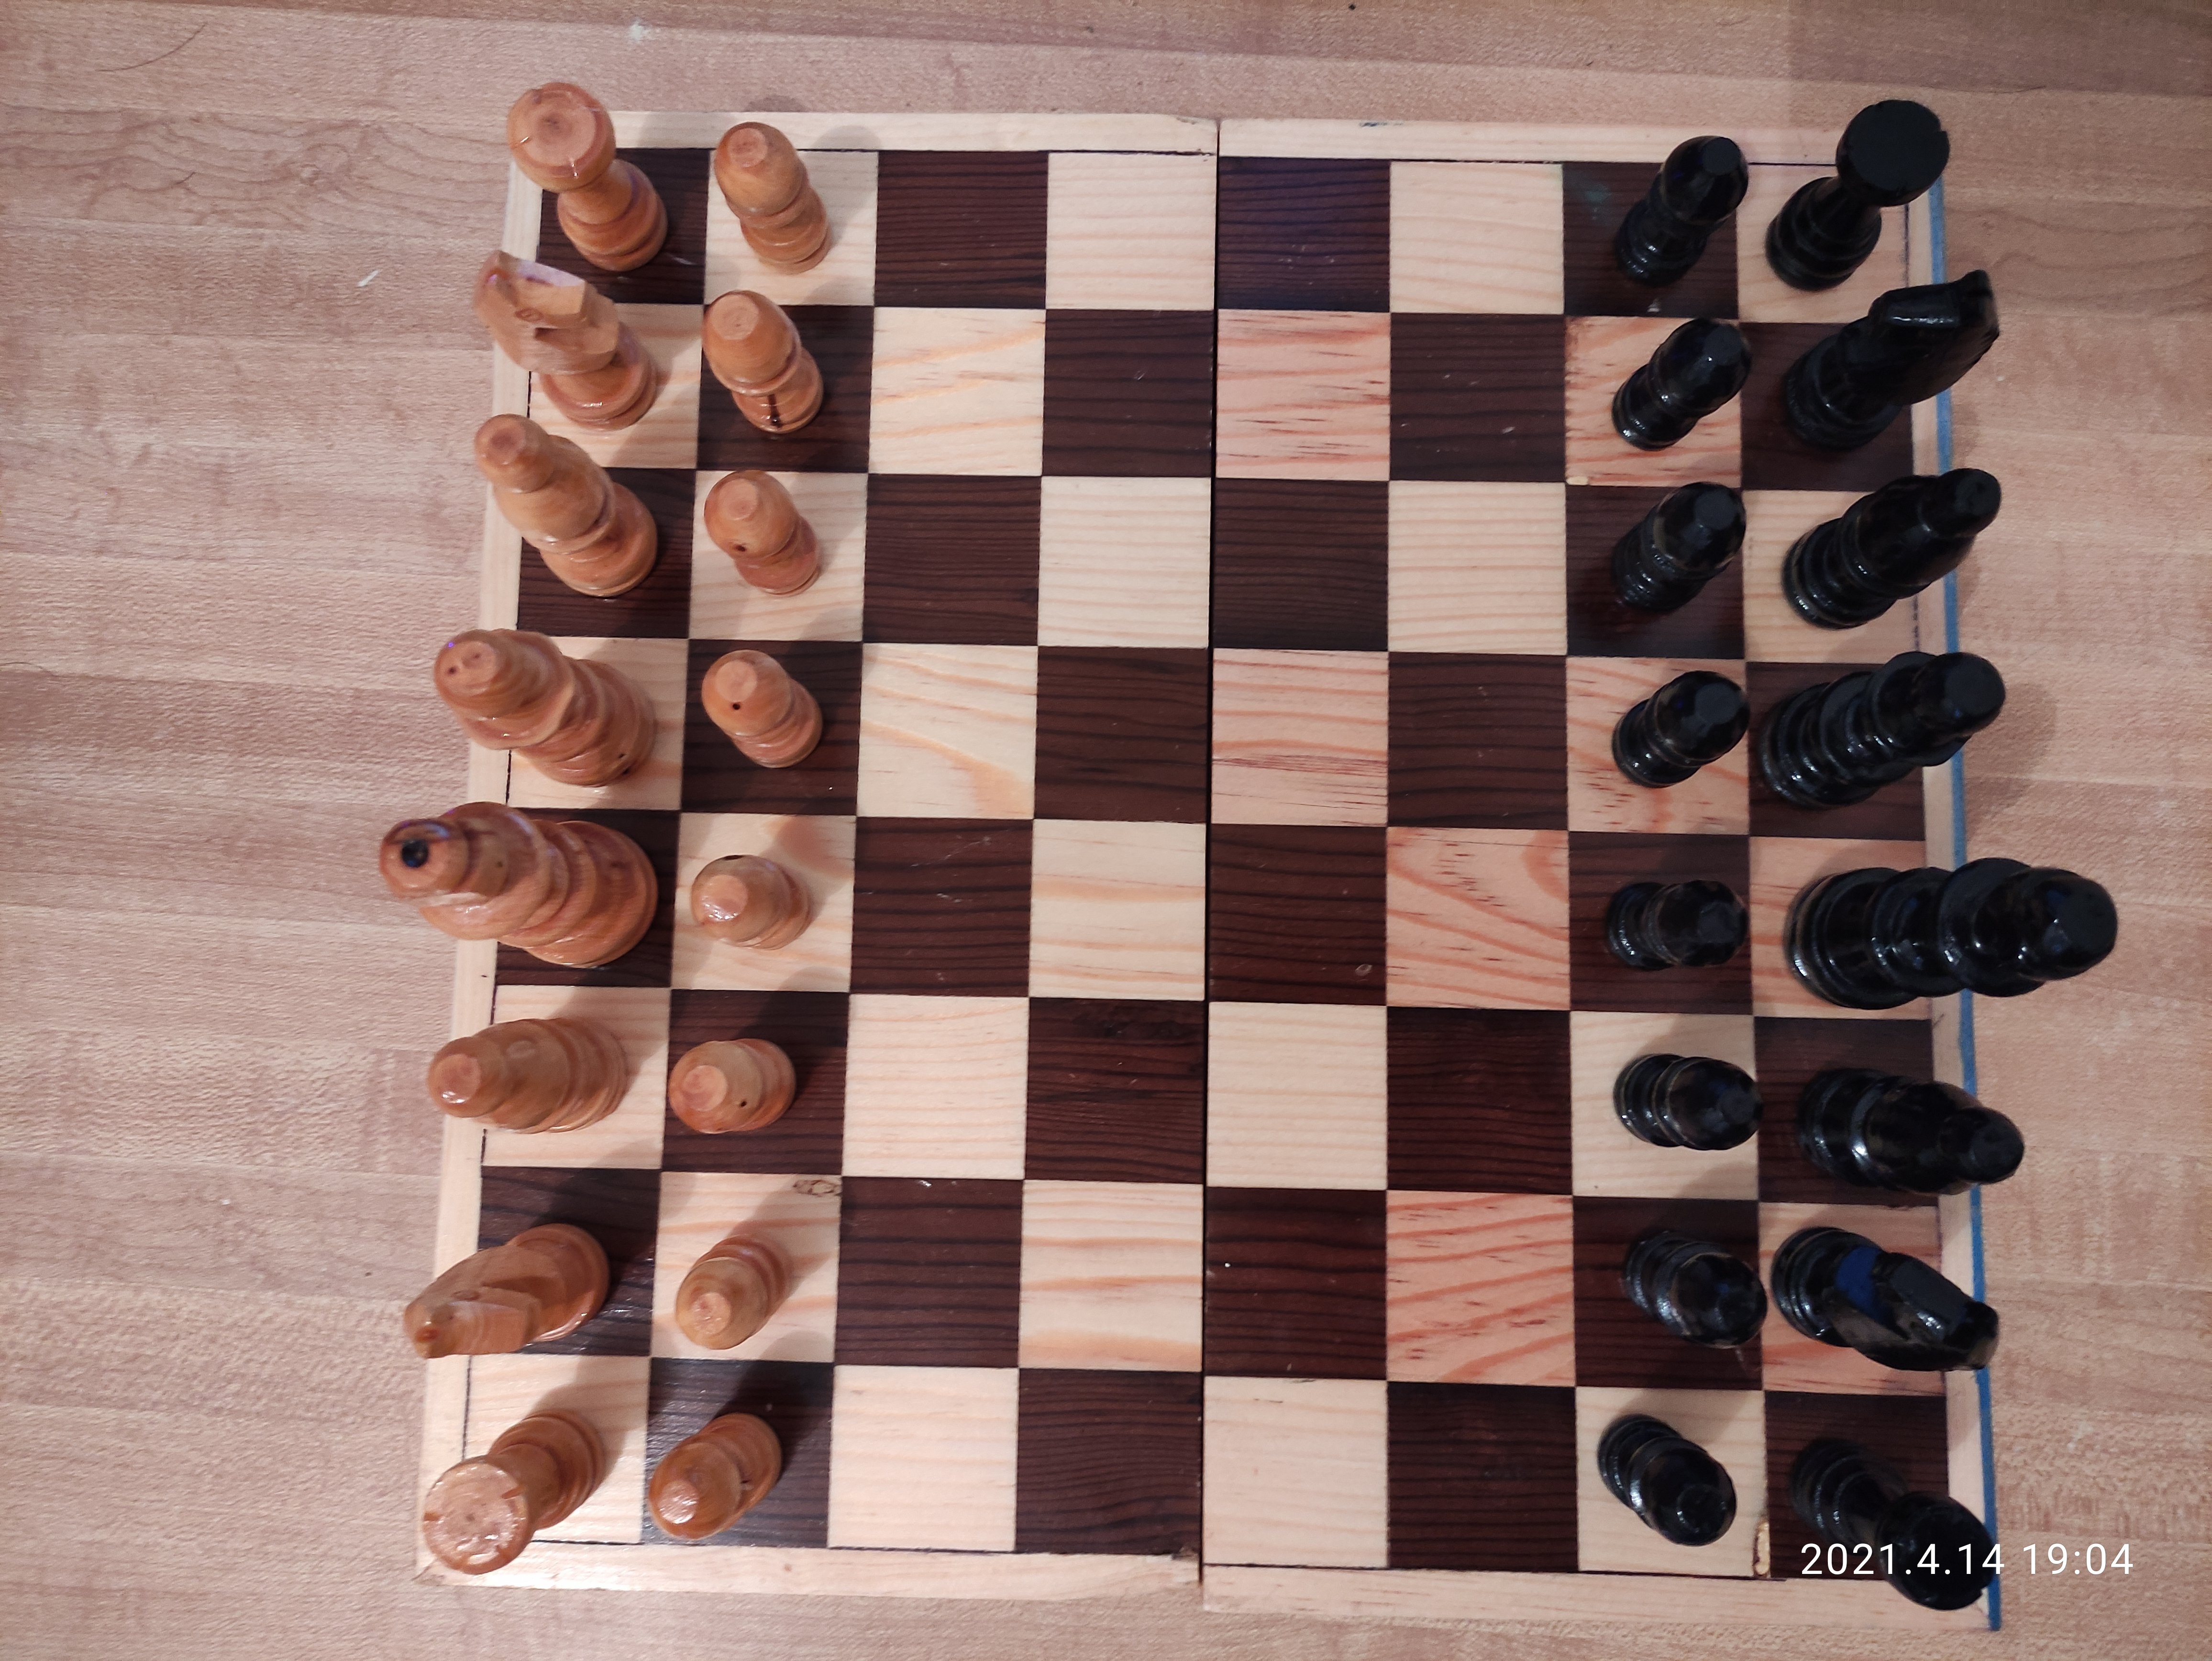
\includegraphics[width=0.75\textwidth]{Figs/AjedrezFroylan2}
     \end{center}
\end{column}

\end{columns}
%\end{block} 
\footnotetext{\fullcite{Froylan_VC_2021}}
%\footnotetext{Froylan Melquiades Wbario Martinez, \textbf{Seguidor de movimientos de Ajedrez}. Universidad Politécnica de Victoria, Informe técnico proyecto de asignatura “Visión por Computadora”, 2021.  En evaluación.}
%\\setcounter{footnote}{0}
\end{frame}

\begin{frame}{Detección de movimientos en un tablero de ajedrez (2)}
%\begin{block}{Detección de movimientos en un tablero de ajedrez (2)} 
\begin{columns}
\begin{column}{0.38\textwidth}
Aplicación de escritorio:
	\begin{itemize}
\item Una vez detectadas las regiones, se emplea un cronometro para determinar la diferencia entre dos instantaneas consecutivas
\item Problemas actuales: Iluminación, sombras, oclusiones
	\end{itemize}
\end{column}
\begin{column}{0.28\textwidth}
\begin{center}
     %%%%% this is a minipage, so \textwidth is already adjusted to the size of the column
     \includegraphics[width=0.79\textwidth]{Figs/AjedrezFroylan3}\\
%     \includegraphics[width=0.49\textwidth]{Figs/AjedrezFroylan4}
     \end{center}
\end{column}
\begin{column}{0.28\textwidth}
\begin{center}
     %%%%% this is a minipage, so \textwidth is already adjusted to the size of the column
%     \includegraphics[width=0.49\textwidth]{Figs/AjedrezFroylan3}\\
     \includegraphics[width=0.79\textwidth]{Figs/AjedrezFroylan4}
     \end{center}
\end{column}

\end{columns}
%\end{block} 
\end{frame}




\section{2022}

\begin{frame}{\citetitle{ProyectoLSM_2022}$^*$  (1)}
\begin{columns}
\begin{column}{0.6\textwidth}
	\begin{itemize}
		\item Se propone una aplicación móvil que reconozca el lenguaje de señas mexicano (LSM)
        \item El equipo capturó videos de los diferentes gestos a clasificar (palabras comunes y letras del alfabeto)
        \item Se utilizó la libreria MediaPipe para la obtención de los marcadores de manos, torso y cabeza
        \item Se entrenó una Red Neuronal Convolucional
	\end{itemize}
\end{column}
\begin{column}{0.4\textwidth}  
\begin{center}
     \begin{tabular}{cc}

         \includegraphics[width=0.98\textwidth]{2022_AplicacionLSM/figs/Diapositiva1.PNG}\\         
      \end{tabular}
\end{center}
\end{column} 
\end{columns} 
\footfullcite*{ProyectoLSM_2022}
\end{frame}


\begin{frame}{\citetitle{ProyectoLSM_2022} (2)}
\begin{columns}
\begin{column}{0.6\textwidth}
Librerías utilizadas:
\begin{itemize}
        \item Tensorflow (PC) y Tensorflow-lite (Smartphone)
		\item MediPipe
	\end{itemize}
Para cada video:
\begin{itemize}
        \item Se normaliza la duración del video a una duración estándard
		\item Se entraen ubicaciones de los marcadores y se estiman angulos
		\item Se anexa al dataset para su posterior entrenamiento
	\end{itemize}
\end{column}
\begin{column}{0.4\textwidth}  
\begin{center}
     \begin{tabular}{c}
         \includegraphics[width=0.98\textwidth]{2022_AplicacionLSM/figs/hand_landmarks.png}\\
          \end{tabular}
\end{center}
\end{column} 
\end{columns} 
\end{frame}

\begin{frame}{\citetitle{ProyectoLSM_2022} (3)}
Una vez entrenada la red, el modelo se incorpora a la aplicación
\begin{center}
 \begin{tabular}{cccc}
    \includegraphics[width=0.16\textwidth]{2022_AplicacionLSM/figs/App1.jpeg}
    \includegraphics[width=0.16\textwidth]{2022_AplicacionLSM/figs/App2.jpeg}
    \includegraphics[width=0.16\textwidth]{2022_AplicacionLSM/figs/Muestra_compañeros1.jpeg}
    \includegraphics[width=0.16\textwidth]{2022_AplicacionLSM/figs/Muestra_compañeros2.jpeg}
  \end{tabular}
\end{center}

\end{frame}








\begin{frame}{\citetitle{MarcoNuno_Revista_2022_03_00}$^*$  (1)}
\begin{columns}
\begin{column}{0.6\textwidth}
	\begin{itemize}
		\item Una solución al problema de manejo de desechos es el reciclado
        \item Específicamente, la separación por color de una botella es de utilidad para su correcto manejo
        \item Se propone un sistema para clasificar botellas en una banda transportadora
        \item El nucleo del sistema es una arquictectura hardware que realiza tareas de visión para clasificación tiempo real 
	\end{itemize}
\end{column}
\begin{column}{0.4\textwidth}  
\begin{center}
     \begin{tabular}{cc}
         \includegraphics[width=0.98\textwidth]{2022_BottleClassifier/figs/MainModules.pdf}\\         
      \end{tabular}
\end{center}
\end{column} 
\end{columns} 
\footfullcite*{MarcoNuno_Revista_2022_03_00}
\end{frame}


\begin{frame}{\citetitle{MarcoNuno_Revista_2022_03_00} (2)}
\begin{columns}
\begin{column}{0.5\textwidth}

Materiales:
\begin{itemize}
        \item Sensor óptico de presencia
        \item Tarjeta FPGA - Spartan 6 Industrial Video Processing Kit
        \item Cámara con salida HDMI
        \item Monitor para depuración
        \item Circuitos para activar actuadores de separación de botellas
	\end{itemize}
\end{column}
\begin{column}{0.5\textwidth}  
\begin{center}
     \begin{tabular}{c}
         \includegraphics[width=0.98\textwidth]{2022_BottleClassifier/figs/cap4_setup.png}\\
          \end{tabular}
\end{center}
\end{column} 
\end{columns} 
\end{frame}

\begin{frame}{\citetitle{MarcoNuno_Revista_2022_03_00} (3)}
El nucleo del sistema propuesto es el módulo del sistema de visión, que ejecuta las siguientes tareas:
\begin{itemize}
        \item Aplicar filtros (promediado y de mediana)
        \item Convertir de Color a HSV
        \item Efectuar operaciones morfológica
        \item Calcular histograma
        \item En base a reglas previamente definidas, clasifica la botella por color
	\end{itemize}

%\begin{center}
% \includegraphics[width=0.95\textwidth]{2022_ConteoOstioncitos/figs/ImageMatchingAndRegistration.png}
%\end{center}

\end{frame}


\begin{frame}{\citetitle{MarcoNuno_Revista_2022_03_00} (4)}
\begin{columns}
\begin{column}{0.6\textwidth}
\begin{itemize}
\item Una vez que el sensor óptico detecta la botella, inicia el procesamiento de imágen
\item Cuando el procesamiento de imágen termina, arroja como resultado la clasificación de la botella
\item Se incrementa un contador de cada botella y se muestra en la pantalla de depuración
\item Es posible configurar los umbrales, para separar botellas de diferente color diferentes
\end{itemize}
\end{column} 
\begin{column}{0.3\textwidth}
 \begin{tabular}{c}
    \includegraphics[width=0.98\textwidth]{2022_BottleClassifier/figs/cap4_dispfinal.png}\\
    \includegraphics[width=0.98\textwidth]{2022_BottleClassifier/figs/cap4_disporiginal.png}
  \end{tabular}
\end{column} 
\end{columns} 

\end{frame}




  

%\begin{frame}{\citetitle{MarcoNuno_ReporteTecnico2022}  \footnotemark{} (1)}
%\begin{frame}{\citetitle{MarcoNuno_ReporteTecnico2022}  \footnote{\fullcite{MarcoNuno_ReporteTecnico2022}} (1)}
\begin{frame}{\citetitle{MarcoNuno_ReporteTecnico2022}$^*$ (1)}
%\begin{frame}{}
%\footfullcite*{MarcoNuno_ReporteTecnico2022}
\begin{columns}
\begin{column}{0.6\textwidth}
	\begin{itemize}  %del cuerpo académico Acuicultura Sustentable (UTMTB-CA-1)
        \item Proyecto desarrollado  en colaboración con investigadores de la Universidad Tecnológica del Mar de Tamaulipas Bicentenario (UTMarT)
		\item Desarrollar una herramienta para automatizar el conteo de microalgas, específicamente de las especies \textit{Isochrysis galbana} e \textit{Chaetoceros muelleri}
        \item Herramientas Software a utilizar: Python (PC), OpenCV, y Android Studio
        \item Herramientas Hardwware a utilizar: Teléfono inteligente (para captura imágenes), adaptador teléfono-microscopio
	\end{itemize}
\end{column}
\begin{column}{0.4\textwidth}  
\begin{center}
     \begin{tabular}{cc}
         \includegraphics[width=0.68\textwidth]{2022_ConteoMicroAlgas/figs/MicroAlgas01}\\         
      \end{tabular}
\end{center}
\end{column} 
\end{columns} 


%\footnotetext[1]{\fullcite{MarcoNuno_ReporteTecnico2022}}
%\setcounter{footnote}{0}
%\footnotetext{\fullcite{MarcoNuno_ReporteTecnico2022}}
%\footfullcite{MarcoNuno_ReporteTecnico2022}
\footfullcite*{MarcoNuno_ReporteTecnico2022}
\end{frame}


\begin{frame}{\citetitle{MarcoNuno_ReporteTecnico2022} (2)}
\begin{columns}
\begin{column}{0.6\textwidth}
Problemas Encontrados:
\begin{itemize}
        \item Rotación de la rejilla de referencia
        \item Nivel de acercamiento es variable
		\item Imágenes con ruido, distancia de captura variable, regionres con desenfoque 
        \item Problemas de contraste (complica encontrar las lineas)
        \item Cuando hay muchas algas, hay grupos de algas que suelen formar lineas falsas
	\end{itemize}
\end{column}
\begin{column}{0.4\textwidth}  
\begin{center}
     \begin{tabular}{cc}
         \includegraphics[width=0.38\textwidth]{2022_ConteoMicroAlgas/figs/CuadranteA}&
         \includegraphics[width=0.38\textwidth]{2022_ConteoMicroAlgas/figs/CuadranteB}\\
         \includegraphics[width=0.38\textwidth]{2022_ConteoMicroAlgas/figs/CuadranteC}&
         \includegraphics[width=0.38\textwidth]{2022_ConteoMicroAlgas/figs/CuadranteD}\\
          \end{tabular}
\end{center}
\end{column} 
\end{columns} 
\end{frame}


\begin{frame}{\citetitle{MarcoNuno_ReporteTecnico2022} (3)}
\begin{columns}
\begin{column}{0.50\textwidth}
Fases del algoritmo en desarrollo:
\begin{itemize}
		\item Binalizar las imágenes y aplicar un algoritmo de detección de bordes
        \item Encontrar las líneas mediante los algoritmos de Hough Standard y Probabilístico
        \item Analizar las líneas encontradas para determinar aquellas que deben descartarse 
        \item Efectuar un enmascarado de regiones para aislar solo la rejilla delimitadora
        \item Llevar a cabo el conteo de las algas a partir de los contornos de la imágen de bordes
	\end{itemize}
\end{column}
\begin{column}{0.50\textwidth}  
\begin{center}
     \begin{tabular}{ccc}
         \includegraphics[width=0.31\textwidth]{2022_ConteoMicroAlgas/figs/MicroAlgas01}&
         \includegraphics[width=0.31\textwidth]{2022_ConteoMicroAlgas/figs/02_Canny}&
         \includegraphics[width=0.31\textwidth]{2022_ConteoMicroAlgas/figs/03_LineasEstandar}\\
         \includegraphics[width=0.31\textwidth]{2022_ConteoMicroAlgas/figs/04_LineasProbabilistico}&
         \includegraphics[width=0.31\textwidth]{2022_ConteoMicroAlgas/figs/05_Delimitacion}&
         \includegraphics[width=0.31\textwidth]{2022_ConteoMicroAlgas/figs/07_ResultadoConteo}\\

          \end{tabular}
\end{center}
\end{column} 
\end{columns} 
\end{frame}



\begin{frame}{\citetitle{MarcoNuno_ReporteTecnico2022} (4)}

\begin{itemize}
\item Hay un avance significativo con respecto al prototipo versión PC (cerca de completarse)
\begin{itemize} 
\item Se requieren más imágenes, que incluyan el conteo realizado de manera manual para contrastarlo con nuestros algoritmos
\item Posiblemente se deban afinar los algoritmos que se tienen desarrollados
\end{itemize}
\item Con respecto a la fase en el teléfono inteligente, se lleva un avance del 20\%, a reserva de la incorporación de un estudiante de estancia o estadía
\item Los resultados apuntan que es posible publicar los resultados en una Revista Indexada por el JCR
\end{itemize}
\end{frame}




      

\begin{frame}{\citetitle{Plagio_Marlly2022}$^*$  (1)}
\begin{columns}
\begin{column}{0.6\textwidth}
	\begin{itemize}
		\item El plagio es un común denominador en diferentes niveles educativos
        \item Se propone un sistema que analiza un conjunto de documentos y detecta plagio mediante diferentes enfoques:
		\begin{itemize}
		\item Analizar el texto de dichos documentos y compararlos entre sí
		\item Extraer y analizar las imágenes y compararlas entre sí
		\end{itemize}
	\end{itemize}
\end{column}
\begin{column}{0.4\textwidth}  
\begin{center}
     \begin{tabular}{c}
\includegraphics[width=0.78\textwidth]{2022_Plagio/figs/P1}\\ \hline
\includegraphics[width=0.78\textwidth]{2022_Plagio/figs/P2}\\         
      \end{tabular}
\end{center}
\end{column} 
\end{columns} 
\footfullcite*{Plagio_Marlly2022}
\end{frame}


\begin{frame}{\citetitle{Plagio_Marlly2022} (2)}
	\begin{itemize}
        \item La aplicación esta codificada en Python, hace uso de OpenCV para comparar imágenes y la librería \textit{TfidVectorizer} para comparación de textio
        \item Una vez efectuado el análisis, se reportan los resultados
	\end{itemize}
\begin{center}
 \begin{tabular}{c}
    \includegraphics[width=0.64\textwidth]{2022_Plagio/figs/analisis.jpg}
  \end{tabular}
\end{center}

\end{frame}







%\begin{frame}{\citetitle{MarcoNuno_ReporteTecnico2022_C} \footnotemark[2] (1)}
\begin{frame}{\citetitle{MarcoNuno_ReporteTecnico2022_C}$^*$  (1)}
%\begin{frame}{---}
%\footfullcite*{MarcoNuno_ReporteTecnico2022_C}

\begin{columns}
\begin{column}{0.70\textwidth}
	\begin{itemize}
		\item Una vez que los ostiones han sido reproducidos, se requiere llevar un registro de su crecimiento mediante conteo. 
        \item Herramientas Software a utilizar: Python (PC), OpenCV, y Android Studio
        \item Herramientas Hardwware a utilizar: Teléfono inteligente (para captura imágenes), adaptador teléfono-microscopio
	\end{itemize}
\end{column}
\begin{column}{0.30\textwidth}  
\begin{center}
     \begin{tabular}{cc}
         \includegraphics[width=0.68\textwidth]{2022_ConteoOstioncitos/figs/R0063.png}\\         
      \end{tabular}
\end{center}
\end{column} 
\end{columns} 


%\footnotetext[1]{\fullcite{MarcoNuno_ReporteTecnico2022_C}}
%\setcounter{footnote}{0}
%\footnotetext{\fullcite{MarcoNuno_ReporteTecnico2022_C}}
%\footfullcite{MarcoNuno_ReporteTecnico2022_C}
\footfullcite*{MarcoNuno_ReporteTecnico2022_C}
\end{frame}


\begin{frame}{\citetitle{MarcoNuno_ReporteTecnico2022_C} (2)}
\begin{columns}
\begin{column}{0.38\textwidth}
Problemas Encontrados:
\begin{itemize}
        \item Iluminación variable
        \item Ruido
	\end{itemize}
\textbf{Entrada}: Una secuencia de imágenes continua (video) en donde el técnico manipula la platina para abarcar un número de muestras mayor
\end{column}
\begin{column}{0.64\textwidth}  
\begin{center}
     \begin{tabular}{c}
         \includegraphics[width=0.24\textwidth]{2022_ConteoOstioncitos/figs/R0078.png}
         \includegraphics[width=0.24\textwidth]{2022_ConteoOstioncitos/figs/R0090.png}
         \includegraphics[width=0.24\textwidth]{2022_ConteoOstioncitos/figs/R0102.png}
         \includegraphics[width=0.24\textwidth]{2022_ConteoOstioncitos/figs/R0126.png}\\
          \end{tabular}
\end{center}
\end{column} 
\end{columns} 
\end{frame}

\begin{frame}{\citetitle{MarcoNuno_ReporteTecnico2022_C} (3)}



Etapas del algoritmo en desarrollo:
\begin{itemize}
        \item Encontrar los puntos característicos y los descriptores de caracteristícas, y estimar una correspondencia
        \item A partir de la correspondencia, estimar la matriz de Homografía y llevar a cabo transformación de tipo Warp para estimar el empalme de imágenes
	\end{itemize}

\begin{center}
 \includegraphics[width=0.95\textwidth]{2022_ConteoOstioncitos/figs/ImageMatchingAndRegistration.png}
\end{center}

\end{frame}


\begin{frame}{\citetitle{MarcoNuno_ReporteTecnico2022_C} (4)}
\begin{center}
 \begin{tabular}{c}
         \includegraphics[width=0.24\textwidth]{2022_ConteoOstioncitos/figs/0049.png}
         \includegraphics[width=0.24\textwidth]{2022_ConteoOstioncitos/figs/0085.png}
         \includegraphics[width=0.24\textwidth]{2022_ConteoOstioncitos/figs/0193.png}
         \includegraphics[width=0.24\textwidth]{2022_ConteoOstioncitos/figs/0373.png}\\
          \end{tabular}
\end{center}
\end{frame}



\begin{frame}{\citetitle{MarcoNuno_ReporteTecnico2022_C} (5)}
Resultado final de la generación del mosaico y del conteo de ostiones
\begin{center}
 \begin{tabular}{c}
         \includegraphics[width=0.50\textwidth]{2022_ConteoOstioncitos/figs/ConteoOstionesFinal.png}\\
          \end{tabular}
\end{center}

\end{frame}



\begin{frame}{\citetitle{MarcoNuno_ReporteTecnico2022_C} (6)}

\begin{itemize}
\item Hay un avance significativo con respecto al prototipo versión PC (cerca de completarse)
\begin{itemize} 
\item Se requieren más imágenes, que incluyan el conteo realizado de manera manual para contrastarlo con nuestros algoritmos
\item Posiblemente se deban afinar los algoritmos que se tienen desarrollados
\end{itemize}
\item Con respecto a la fase en el teléfono inteligente, se lleva un avance del 10\%, a reserva de la incorporación de un estudiante de estancia o estadía
\item Los resultados apuntan que es posible publicar los resultados en una Revista Indexada por el JCR
\end{itemize}




\end{frame}



    

\section{2023}

\renewcommand{\EntradaBibtex}{AppComidaTamaulipeca_SistemasInteligentes_UPV_2023}


\begin{frame}{\citetitle{\EntradaBibtex} \footnotemark[1] (1)}
\begin{block}{Motivación} 
Desarrollar aplicación enfocada en la comida de una región para obtener información nutricional de la misma
\end{block} 
\begin{itemize}
\item Crear un modelo entrenado (usando TensorFlow) con imágenes de comida (gorditas, flautas, tamales, tortas y pozole)
\item Integar dicho modelo a una aplicación móvil (en Android) 
\item Al tomar una foto con la aplicación, se indique de que alimento se trata, además de su información nutrimental
\end{itemize}
\footnotetext[1]{\fullcite{\EntradaBibtex}}
\end{frame}

\begin{frame}{\citetitle{\EntradaBibtex} (2)}

\begin{center}
	\begin{tabular}{ccccc}
		\includegraphics[width=0.18\linewidth,height=4.85cm]{2023_AppComidaTamaulipeca/figs/AppComida1.png} &
		\includegraphics[width=0.18\linewidth,height=4.85cm]{2023_AppComidaTamaulipeca/figs/AppComida2.png} &
		\includegraphics[width=0.18\linewidth,height=4.85cm]{2023_AppComidaTamaulipeca/figs/AppComida3.png} &
		\includegraphics[width=0.18\linewidth,height=4.85cm]{2023_AppComidaTamaulipeca/figs/AppComida4.png} &
		\includegraphics[width=0.18\linewidth,height=4.85cm]{2023_AppComidaTamaulipeca/figs/AppComida5.png}  \\
	\end{tabular}
\end{center}

\end{frame}

%





\renewcommand{\EntradaBibtex}{MarcoNuno_Revista_2023_09_00}

\begin{frame}{\citetitle{\EntradaBibtex}$^*$ (1)}
\begin{block}{Motivación} 
Tamaulipas es uno de los principales productores de cítricos. Mucho de la separación de la producción se hace aún de manera manual
\end{block} 
Se propone un sistema de alto desempeño para separar los citricos en una banda transportadora.
\begin{itemize}
\item Se utilizó un FPGA (Spartan6 Industrial Video Processing Kit) y el lenguaje de programación VHDL
\item La cámara está ubicada en un compartimiendo con luz controlada
\item Se efectúa la separación por tamaño y por nivel de madurez
\end{itemize}
\footfullcite*{\EntradaBibtex}
\end{frame}


\begin{frame}{\citetitle{\EntradaBibtex} (2)}
%\begin{block}{Pantallas Principales} 
\begin{center}
	\begin{tabular}{ccc}
		\includegraphics[width=0.25\linewidth]{2023_ConteoNaranjasBandaTransportadora/figs/ImagenBanda.png} &
		\includegraphics[width=0.25\linewidth]{2023_ConteoNaranjasBandaTransportadora/figs/interior.png} &
		\includegraphics[width=0.45\linewidth]{2023_ConteoNaranjasBandaTransportadora/figs/ImagenTablero.png} \\
	\end{tabular}
\end{center}
\end{frame}


\begin{frame}{\citetitle{\EntradaBibtex} (3)}
%\begin{block}{Pantallas Principales} 
\begin{center}
	\begin{tabular}{c}
		\includegraphics[width=0.65\linewidth]{2023_ConteoNaranjasBandaTransportadora/figs/Figura_ArticuloAntonio_MainSystem_VersionESL.png} \\
	\end{tabular}
\end{center}
\end{frame}



\begin{frame}{\citetitle{\EntradaBibtex} (4)}
%\begin{block}{Pantallas Principales} 
\begin{center}
	\begin{tabular}{ccc}
		\includegraphics[width=0.45\linewidth]{2023_ConteoNaranjasBandaTransportadora/figs/framito.png} &
		\includegraphics[width=0.25\linewidth]{2023_ConteoNaranjasBandaTransportadora/figs/blur.png} &
		\includegraphics[width=0.25\linewidth]{2023_ConteoNaranjasBandaTransportadora/figs/blurmask.png} \\
	\end{tabular}
\end{center}
\end{frame}


\begin{frame}{\citetitle{\EntradaBibtex} (5)}
\begin{itemize}
\item Es posible obtener precisiones de 94\% con respecto al color y 96\% con respecto al tamaño 
\item El sistema ya acoplado con la banda transportadora puede clasificar hasta 5 naranjas por segundo (3.6 toneladas por hora)
\item La principal limitante de la velocidad de clasificación son los elementos mecánicos (banda transportadora, actuadores, etc). El sistema de visión en teoría puede procesar 60 naranjas por segundo (43.2 toneladas por hora)
\end{itemize}

\end{frame}




\renewcommand{\EntradaBibtex}{AppSegmentaCromosomas_SistemasInteligentes_UPV_2023}


\begin{frame}{\citetitle{\EntradaBibtex} \footnotemark[1] (1)}
\begin{block}{Motivación} 
Desarrollar aplicación móvil para que el Citogenetista localice los cromosomas en imágenes de estudios de citogenética y genere el Cariograma
\end{block} 
\begin{itemize}
\item El usario selecciona una carpeta con imágenes de cromosomas y la imagen de trabajo. 
\item Se incluyen funciones de paneo y acercamiento/alejamiento
\item Con el dedo hacer trazos sobre los cromosomas (definir el esqueleto). Personalizar el grosor y el color del trazo.
\item Una vez finalizado el trazo pregunta el número de cromosoma recién seleccionado (23 pares de cromosomas)
\item Al seleccionar todos los cromosomas, generar el Cariograma
\end{itemize}
\footnotetext[1]{\fullcite{\EntradaBibtex}}
\end{frame}

\begin{frame}{\citetitle{\EntradaBibtex} (2)}

\begin{center}
	\begin{tabular}{ccccc}
		\includegraphics[width=0.18\linewidth,height=4.85cm]{2023_AppSegmentaCromosomas/figs/vistadeimagen.jpg}  &
		\includegraphics[width=0.18\linewidth,height=4.85cm]{2023_AppSegmentaCromosomas/figs/trazado.jpg} &		
		\includegraphics[width=0.18\linewidth,height=4.85cm]{2023_AppSegmentaCromosomas/figs/ediciondetrazo.jpg} &
		\includegraphics[width=0.18\linewidth,height=4.85cm]{2023_AppSegmentaCromosomas/figs/archivosdescargados.jpg} &
		\includegraphics[width=0.18\linewidth,height=4.85cm]{2023_AppSegmentaCromosomas/figs/cariograma.png} \\
	\end{tabular}
\end{center}

\end{frame}


\begin{frame}{\citetitle{\EntradaBibtex} (3)}

\begin{center}
		\includegraphics[width=0.70\linewidth]{2023_AppSegmentaCromosomas/figs/AppCromosomasTablet.png}  
\end{center}

\end{frame}


%




\renewcommand{\EntradaBibtex}{AplicacionMovilManoRobotica_SistemasInteligentes_UPV_2023}


\begin{frame}{\citetitle{\EntradaBibtex} \footnotemark[1] (1)}
\begin{block}{Propuesta} 
Un modelo 3D dinámico de una Mano controlado por el usuario implementado en un teléfono inteligente
\end{block} 
\begin{itemize}
\item Utiliza la cámara del teléfono inteligente para detectar la mano (Libreria MediaPipe)
\item Utiliza OpenGL ES para crear el entorno 3D de una mano humana modelada en Blender
\item En base a los movimientos de los dedos del usuario, el modelo se actualiza
\end{itemize}
\footnotetext[1]{\fullcite{\EntradaBibtex}}
\end{frame}

\begin{frame}{\citetitle{\EntradaBibtex} (2)}

\begin{center}
	\begin{tabular}{ccc}
		\includegraphics[width=0.20\linewidth]{2023_ManoRobotica/figs/hand01.jpeg} &
		\includegraphics[width=0.20\linewidth]{2023_ManoRobotica/figs/hand02.jpeg} & 
		\includegraphics[width=0.20\linewidth]{2023_ManoRobotica/figs/hand03.jpeg}\\
	\end{tabular}
\end{center}

\end{frame}

%




\renewcommand{\EntradaBibtex}{ClasificadorHabaneros_ProcesadoresDigitales_UPV_2023}


\begin{frame}{\citetitle{\EntradaBibtex}$^*$ (1)}
\begin{block}{Propuesta} 
Una aplicación que clasifique chiles habaneros por su grado de madurez
\end{block} 
\begin{itemize}
\item Se creó un dataset con 3 niveles de madurez (verde, amarillo y rojo) y un nivel ``No-Chile''
\item Se codificó una aplicación que permite al usuario seleccionar regiones rectangulares de una imagen y asignarles el nivel de madurez de manera manual
\item Se entrenaron diferentes modelos para obtener el de mejor desempeño
\item La idea a futuro es integrar este clasificador con un sistema hidropónico para monitorear de manera remota un cultivo y establecer el tiempo de cosecha optimo de cada chile.
\end{itemize}
\footfullcite*{\EntradaBibtex}
\end{frame}

\begin{frame}{\citetitle{\EntradaBibtex} (2)}

\begin{center}
	\begin{tabular}{ccc}
		\includegraphics[width=0.20\linewidth]{2023_ChilesHabaneros/figs/im1.png} &
		\includegraphics[width=0.75\linewidth]{2023_ChilesHabaneros/figs/Mosaico.png} & \\
	\end{tabular}
\end{center}

\end{frame}

%




\section{2024}

\renewcommand{\EntradaBibtex}{ConteoMonedasAppMovil_SistemasInteligentes_UPV_2023}

\begin{frame}{\citetitle{\EntradaBibtex} \footnotemark[1] (1)}
\begin{block}{Motivación} 
Se requiere migrar la aplicación móvil para conteo de monedas
\begin{itemize}
\item Utiliza la cámara del teléfono inteligente
\item Mismas limitantes de la aplicación de escritorio
\begin{itemize}
\item Las monedas pueden estar encimadas (con cierto grado permisible)
\item Se limitan a monedas de la misma denominación
\end{itemize}
\item Se emplean herramientas para eliminar ruido, detectar circulos
\item Por el momento el usuario solo puede seleccionar un\usepackage[symbol]{footmisc} denominación
\end{itemize}
\end{block} 
\footnotetext[1]{\fullcite{\EntradaBibtex}}
\end{frame}

\begin{frame}{\citetitle{\EntradaBibtex} (2)}

\begin{center}
	\begin{tabular}{cc}
		\includegraphics[width=0.28\linewidth]{2024_ConteoMonedasEscritorio/figs/1.jpeg} &
		\includegraphics[width=0.28\linewidth]{2024_ConteoMonedasEscritorio/figs/4.jpeg} \\

	\end{tabular}
\end{center}
\end{frame}



\renewcommand{\EntradaBibtex}{ConteoMonedasEscritorio_SistemasInteligentes_UPV_2024}

\begin{frame}{\citetitle{\EntradaBibtex} \footnotemark[1] (1)}
\begin{block}{Motivación} 
Se requiere una herramienta para apoyar a pequeños comerciantes en el conteo de su morralla
\begin{itemize}
\item Se requiere una cámara WEB conectada a la computadora, montada en un tripie a cierta altura	
\item Por el momento se requieren condiciones muy particulares (fondo blanco, respectar distancia entre cámara-objetos)
\begin{itemize}
\item Las monedas pueden estar encimadas (con cierto grado permisible)
\end{itemize}
\item Se emplean herramientas para eliminar ruido, detectar circulos
\item Los circulos se ajustan por tamaño para determinar las denominaciones
\item Al final, se genra como resultado el estimado de la cantidad de dinero existente (no sólo el número de monedas)
\end{itemize}
\end{block} 
\footnotetext[1]{\fullcite{\EntradaBibtex}}
\end{frame}


\begin{frame}{\citetitle{\EntradaBibtex} (2)}
%\begin{block}{Pantallas Principales} 

%\begin{columns}
% Column 1
%\column{.8\linewidth}

\begin{center}
	\begin{tabular}{ccc}
		\includegraphics[width=0.32\linewidth]{2024_ConteoMonedasEscritorio/figs/ct1b.jpeg} &
		\includegraphics[width=0.32\linewidth]{2024_ConteoMonedasEscritorio/figs/ct2b.jpeg} & 
		\includegraphics[width=0.36\linewidth]{2024_ConteoMonedasEscritorio/figs/d.jpg}\\
	\end{tabular}
\end{center}

%\column{.1\linewidth}
%\begin{center}%
%	\begin{tabular}{cccc}
%		\includegraphics[width=0.48\linewidth]{2024_DeteccionAlimentosAlbercas/figs/im2.jpg} &
 %		\includegraphics[width=0.48\linewidth]{2024_DeteccionAlimentosAlbercas/figs/im3.jpg} \\
	%	\includegraphics[width=0.48\linewidth]{2024_DeteccionAlimentosAlbercas/figs/im4.jpg} &
 	%	\includegraphics[width=0.48\linewidth]{2024_DeteccionAlimentosAlbercas/figs/im5.jpg} \\
%	\end{tabular}
%\end{center}




%\end{columns}
\end{frame}

%




%\newcommand{\EntradaBibtex}{ConteoNaranjasArboles_UPV_2024}
\renewcommand{\EntradaBibtex}{ConteoNaranjasArboles_UPV_2024}

\begin{frame}{\citetitle{\EntradaBibtex}$^*$ (1)}
\begin{block}{Motivación} 
Se requiere de una herramienta que permita estimar el número de naranjas antes del corte
\begin{itemize}
\item Se implementó una aplicación que permite al usuario seleccionar imágenes
\item Se empleó una red neuronal SSD MobileNet
\item Se utilizaron imágenes con resolución de entrada 320x320 píxeles
\end{itemize}
\end{block} 
\footfullcite*{\EntradaBibtex}
\end{frame}


\begin{frame}{\citetitle{\EntradaBibtex} (2)}
%\begin{block}{Pantallas Principales} 
\begin{center}
	\begin{tabular}{cc}
		\includegraphics[width=0.35\linewidth]{2024_ConteoNaranjasArbol/figs/1.jpg} &
		\includegraphics[width=0.35\linewidth]{2024_ConteoNaranjasArbol/figs/2.jpg} \\ 		 		
		\includegraphics[width=0.35\linewidth]{2024_ConteoNaranjasArbol/figs/3.jpg} & 		
		\includegraphics[width=0.35\linewidth]{2024_ConteoNaranjasArbol/figs/4.jpg} \\
	\end{tabular}
\end{center}
\end{frame}




\renewcommand{\EntradaBibtex}{DetecciónAlimentosEnAlbercas_SistemasInteligentes_UPV_2024}

\begin{frame}{\citetitle{\EntradaBibtex}$^*$ (1)}
\begin{block}{Motivación} 
Se requiere una herramienta para monitorear de manera remota a un grupo de usuarios de una alberca privada
\begin{itemize}
\item Se generardos dos conjuntos de entrenamiento: 
\begin{itemize}
\item Uno que incluye imágenes de albercas
\item Uno que incluye imágenes de personas consumiendo alimentos
\end{itemize}
\item Se entrenan los modelos por separado y posteriormente se combinan para generar la clasificación de salida. Específicamente se emplea el modelo YOLO (You only look once) v5 para detectar las personas con alimentos. 
\end{itemize}
\end{block} 
\footfullcite*{\EntradaBibtex}
\end{frame}


\begin{frame}{\citetitle{\EntradaBibtex} (2)}
%\begin{block}{Pantallas Principales} 

\begin{columns}
% Column 1
\column{.5\linewidth}

\begin{center}
	\begin{tabular}{cc}
		\includegraphics[width=0.48\linewidth]{2024_DeteccionAlimentosAlbercas/figs/val_batch0_pred.jpg} &
		\includegraphics[width=0.48\linewidth]{2024_DeteccionAlimentosAlbercas/figs/val_batch1_labels.jpg} \\
	\end{tabular}
\end{center}

\column{.5\linewidth}
\begin{center}
	\begin{tabular}{cccc}
		\includegraphics[width=0.48\linewidth]{2024_DeteccionAlimentosAlbercas/figs/im2.jpg} &
 		\includegraphics[width=0.48\linewidth]{2024_DeteccionAlimentosAlbercas/figs/im3.jpg} \\
		\includegraphics[width=0.48\linewidth]{2024_DeteccionAlimentosAlbercas/figs/im4.jpg} &
 		\includegraphics[width=0.48\linewidth]{2024_DeteccionAlimentosAlbercas/figs/im5.jpg} \\
	\end{tabular}
\end{center}


\end{columns}
\end{frame}





%/media/marco/Master/00_0A0RespadoLaptopHP_2024/Escritorio/00_DiapositivasProyectos/2024_PaseDeListaCodigoQR/figs/2.jpg
%/media/marco/Master/00_0A0RespadoLaptopHP_2024/Escritorio/00_DiapositivasProyectos/2024_PaseDeListaCodigoQR/figs/3.jpg
%/media/marco/Master/00_0A0RespadoLaptopHP_2024/Escritorio/00_DiapositivasProyectos/2024_PaseDeListaCodigoQR/figs/4.jpg



\input{2024_DetectorMotos/DetectorMotos.tex}

\renewcommand{\EntradaBibtex}{GerminadorAutomatico_EstadiasMecatronica_UPV_2024}

\begin{frame}{\citetitle{\EntradaBibtex}$^*$ (1)}
\begin{block}{Motivación} 
 Un germinador favorece el desarrollo de semillas en condiciones adecuadas (temperatura y humedad). Su automatización es importante para incentivar el cultivo de alimentos en casa
\end{block} 

\begin{itemize}
\item Se agregan sensores, actuadores y software para monitorear el desarrollo de los brotes de manera remota
\item Una cámara captura fotos de los brotes en intervalos de tiempo regulares
\item Los sensores de humedad y temperatura permiten obtener retroalimentación de las condiciones del entorno de los brotes
\item Un sistema de bombeo de agua permite mantener la humedad en niveles óptimos 
\end{itemize}

\footfullcite*{\EntradaBibtex}
\end{frame}

\begin{frame}{\citetitle{\EntradaBibtex} (2)}

\begin{columns}

% Column 1
\column{.6\linewidth}

\begin{center}
	\begin{tabular}{cc}
		\includegraphics[width=0.5\linewidth]{2024_GerminadorAutomatico/figs/PrototipoGerminador.png}&
		\includegraphics[width=0.5\linewidth]{2024_GerminadorAutomatico/figs/GerminadorFinal.png} \\
	\end{tabular}
\end{center}
\column{.4\linewidth}
	\begin{tabular}{c}
		\includegraphics[width=0.9\linewidth]{2024_GerminadorAutomatico/figs/SemillasenGerminador.png} \\
		\includegraphics[width=0.9\linewidth]{2024_GerminadorAutomatico/figs/ModuloVision.png} \\
	\end{tabular}

\end{columns}

\end{frame}

\begin{frame}{\citetitle{\EntradaBibtex} (3)}
\begin{itemize}
	\item Se seleccionaron plantas de rápido crecimiento, con la finalidad de obtener resultados significativos. Específicamente, los cultivos seleccionados fueron frijol, lenteja, cilandro y lechuga.
    %\item El germinador automático permite garantizar un crecimiento saludable de las plantas al monitorear los brotes de manera continua. 
    \item El monitoreo visual remoto facilita la detección temprana de problemas y la toma de decisiones informadas.
    \item El sistema propuesto permitirá la evaluación de las mismas condiciones de temperatura/humedad/iluminación con diferentes variedades de semillas, o variar las condiciones con sobre la misma variedad de semilla.  
    \item Con respecto al módulo de visión, se desea determinar de manera precisa el número de hojas del brote, con la finalidad de indicar al usuario del momento adecuado para hacer el trasplante o se requiera atención especial.
\end{itemize}
\end{frame}






\renewcommand{\EntradaBibtex}{IdentificadorGeneroEspectrogramas_SistemasInteligentes_UPV_2024}

\begin{frame}{\citetitle{\EntradaBibtex}$^*$ (1)}
\begin{block}{Motivación} 
A partir de un audio personal, es posible determinar el género (biológico) de dicha persona
\begin{itemize}
\item Se grabaron audios de ambos generos
\item Se utilizó una librería para obtener su espectrograma
\item Se entrenó un modelo para clasificar imágenes de espectrograma obtenidos del audio grabado mediante la interfaz
\item Se creó una interfaz de usuario que vincula el grabador de sonidos del sistema con el modelo previamente entrenado
\end{itemize}
\end{block} 
\footfullcite*{\EntradaBibtex}
\end{frame}


\begin{frame}{\citetitle{\EntradaBibtex} (2)}
%\begin{block}{Pantallas Principales} 

%\begin{columns}
% Column 1
%\column{.1\linewidth}
%\begin{center}
%\includegraphics[width=0.85\linewidth]{2024_DetectorMotos/figs/resultados1.png}
%\includegraphics[width=0.85\linewidth]{2024_DetectorMotos/figs/resultados2.png}
%\end{center}
%\column{.9\linewidth}
\begin{center}
	\begin{tabular}{ccc} \hline
		Genero & Total de Pruebas & Aciertos \\
\hline
		Masculino & 29 & 23 (79\%) \\
		Femenito  & 23 & 19 (82\%)\\
		Total     & 52 & 42 (80\%)\\
\hline
	\end{tabular}
\end{center}

\begin{center}

	\begin{tabular}{cccc}
		\includegraphics[width=0.20\linewidth]{2024_IdentificadorGeneroEspectrograma/figs/esp1.png} &
		\includegraphics[width=0.20\linewidth]{2024_IdentificadorGeneroEspectrograma/figs/esp3.png} &
		\includegraphics[width=0.20\linewidth]{2024_IdentificadorGeneroEspectrograma/figs/esp2.png} &
		\includegraphics[width=0.20\linewidth]{2024_IdentificadorGeneroEspectrograma/figs/esp4.png} \\
	\end{tabular}
\end{center}

%\end{columns}
\end{frame}



\renewcommand{\EntradaBibtex}{PaseListasCodigoQRFaceDetection_SistemasInteligentes_UPV_2024}

\begin{frame}{\citetitle{\EntradaBibtex}$^*$ (1)}
\begin{block}{Motivación} 
Se requiere una herramienta que permita efectuar un pase de lista efectivo en grupos numerosos. 
\begin{itemize}
\item Se capturan fotografias de los asistentes del grupo, además de asignar a cada alumno de un código QR
\item Se emplea un modelo un módulo de Python denominado \textit{face-recognition} para entrena un modelo de aprendizaje profundo para reconocer los rostros de los asistentes a la clase
\item Se emplea una librería para detección de códigos QR
\item Se cruza la información de la identidad del estudiante con el código QR
\end{itemize}
\end{block} 
\footfullcite*{\EntradaBibtex}
\end{frame}


\begin{frame}{\citetitle{\EntradaBibtex} (2)}
%\begin{block}{Pantallas Principales} 

%\begin{columns}
% Column 1
%\column{.1\linewidth}
%\begin{center}
%\includegraphics[width=0.85\linewidth]{2024_DetectorMotos/figs/resultados1.png}
%\includegraphics[width=0.85\linewidth]{2024_DetectorMotos/figs/resultados2.png}
%\end{center}
%\column{.9\linewidth}
\begin{center}
	\begin{tabular}{ccc}
		\includegraphics[width=0.20\linewidth]{2024_PaseDeListaCodigoQR/figs/2.jpg} &
		\includegraphics[width=0.38\linewidth]{2024_PaseDeListaCodigoQR/figs/3.jpg} &
 		\includegraphics[width=0.38\linewidth]{2024_PaseDeListaCodigoQR/figs/4.jpg} \\
	\end{tabular}
\end{center}

%\end{columns}
\end{frame}

%/media/marco/Master/00_0A0RespadoLaptopHP_2024/Escritorio/00_DiapositivasProyectos/2024_PaseDeListaCodigoQR/figs/2.jpg
%/media/marco/Master/00_0A0RespadoLaptopHP_2024/Escritorio/00_DiapositivasProyectos/2024_PaseDeListaCodigoQR/figs/3.jpg
%/media/marco/Master/00_0A0RespadoLaptopHP_2024/Escritorio/00_DiapositivasProyectos/2024_PaseDeListaCodigoQR/figs/4.jpg




\renewcommand{\EntradaBibtex}{MarcoNuno_ReporteTecnico2024}

\begin{frame}{\citetitle{\EntradaBibtex}$^*$ (1)}
\begin{block}{Motivación} 
Es necesario automatizar el proceso de evaluación a nivel estatal de estudiantes de nivel medio superior
\end{block} 

\begin{itemize}
\item Se tuvo acceso a un repositorio de 6000 imágenes de digitalizaciones de examenes
\item Detectar los reactivos asignados de manera exacta (con el mínimo de errores) y generar un Excel con dicha información
\item Problemas: Variación en la iluminación, errores en el escaneo, forma de rellenar el circulo por parte de los estudiantes, etc.
\item Estos reactivos alimentan a otro sistema para obtener el resultado de la evaluación
\end{itemize}

\footfullcite*{\EntradaBibtex}
\end{frame}


\begin{frame}{\citetitle{\EntradaBibtex} (2)}
\begin{columns}

% Column 1
\column{.75\linewidth}
\begin{itemize}
\item Detectar rectangulos contenedores. Identificador (Superior) y Respuestas (Inferior)
\item Para los IDs:
\begin{itemize}
\item Se analiza por filas para obtener el ID
\item Opciones para cada fila del ID: 0-9, en blanco (X) o múltiple (M)
\item 4607 para el exámen mostrado
\end{itemize}
\item Para las respuestas:
\begin{itemize}
\item Deliminar una rejilla en donde se infieren están los aciertos.
\item Opciones para el acierto: A/B/C/D, en blanco (X) o múltiple (M)
\end{itemize}
\end{itemize}
\column{.25\linewidth}
	\begin{center}
	%\begin{tabular}{cc}
		\includegraphics[width=0.90\linewidth]{2024_ProyectoCalificadorExamenes/figs/ExamenES1.png}
		%\includegraphics[width=0.20\linewidth]{2024_ProyectoCalificadorExamenes/figs/ExamenES1.png} \\
	%\end{tabular}
\end{center}

\end{columns}

\end{frame}


\begin{frame}{\citetitle{\EntradaBibtex} (3)}
Problemas Detectados
\begin{center}
	\begin{tabular}{ccc}
		\includegraphics[width=0.35\linewidth]{2024_ProyectoCalificadorExamenes/figs/CasoFlojera.png}&
		\includegraphics[width=0.10\linewidth]{2024_ProyectoCalificadorExamenes/figs/CasosBorrosos.png} &
		\includegraphics[width=0.15\linewidth]{2024_ProyectoCalificadorExamenes/figs/RespuestaMultiple.png} \\
		Circulos no completos & Borrado de respuesta & Respuesta Multiple \\ 

	\end{tabular}
\end{center}
Estado:
\begin{itemize}
\item Se está evaluando la precisión del sistema (Se estima por arriba del 95\%)
\item Se generó una interfaz para seleccionar carpetas de examenes. Organizados por centro de institucion y semestre (2do, 4to y 6to) y se genera el archivo de Excel con las respuestas
\end{itemize}



\end{frame}





\section[CP1]{Conclusiones}
\begin{frame}{Conclusi\'on}
\begin{itemize}
\item Se present\'o la relaci\'on entre Inteligencia Articial, Visi\'on por Computadora y los Gr\'aficos por Computadora con la RA y la RV
\item Se establecieron las herramientas Hardware y Software para Realizar proyectos Gr\'aficos y de RA y RV para Tel\'efonos Inteligentes en Android Studio
\item Se presentaron proyectos de Graficaci\'on y de RA y RV, principalmente desarrollados por estudiantes de la UPV (Ingenier\'ia en Tecnolog\'ias de la Informaci\'on y de Maestría en Ingeniería)
%\item Algunos trabajos establecen vínculos de colaboracion con otras universidades
\end{itemize}
\end{frame}





\renewcommand*{\bibfont}{\tiny}
\begin{frame}[allowframebreaks]{Artículos publicados}
    \printbibliography[title=Artículos publicados,keyword=primary]
\end{frame}

\end{document}


